\section{Introduction}\label{sec:introduction-results}
This section is covering experiments results that were gotten in this case study.
The main idea behind benchmarks and metrics in the case study is to understand
the following details:

\begin{itemize}
    \item How fast two systems recover from unexpected faults.
    \item Partition balancing behavior in case of unexpected faults.
    \item How much network traffic do systems use.
    \item How much CPU is used to find most effective nodes for workers, production cost depends on the type of nodes.
\end{itemize}

All experiments were executed in Kubernetes environments, which means all replicas that
get periodically killed by Chaos Mesh automatically restarted by Kubernetes.
Both prototypes based on Kafka Streams and Apache Flink use the same Kafka records
commit time which is 2 seconds for all experiments.
Such record commit time is supposed to achieve similar stateful streaming behavior
for both prototypes.
For this case study were chosen two main scenarios, when 2 of 8 cluster workers are down for
a short period and when all workers 8 of 8 are down.
Such scenarios should give an overview about how two systems behave if part of workers
get down and a whole worker cluster.


\begin{itemize}
    \item Kafka Streams with having 8 worker replicas killed every 3 minutes
    \item Kafka Streams with having 2 worker replicas killed every 3 minutes
    \item Apache Flink with having 2 worker replicas killed every 3 minutes
    \item Apache Flink with having 8 worker replicas killed every 3 minutes
\end{itemize}

For each experiment were chosen the following parameters:

\begin{description}
    \item[Workers] 8 replicas
    \item[Experiment execution time] 18 minutes
    \item[Records per second] 200000
    \item[Record size] 1KB
    \item[Number of Kafka topic partitions] 50
    \item[Chaos Mesh failure period] 3 minutes
    \item[Number of states] 1000
    \item[Kafka Streams commit time] 2 seconds
    \item[Apache Flink checkpoint save period] 2 seconds
\end{description}



\subsection{Benchmarks}\label{subsec:definition-of-benchmarks}

\begin{description}
    \item[Input Records per Second] records that are coming from a Kafka input topic.
    \item[Output Records per Second] processed records that get sent to a Kafka output topic.
    \item[Lag Trend] denotes the difference between the last record produced by the producer and the offset committed by the consumer group.
    Defines how fast a cluster of workers is able to process an incoming load from a Kafka input topic.
    Such a benchmark combines all partitions that are assigned to a workers consumer group.
    \item[Lag Trend per Partition] denotes Lag trend for each partition separately.
    \item[CPU Utilization] denotes how much CPU worker node consumes during the experiment in percentages.
    \item[Network Recevied] denotes how much network traffic in MB worker nodes received during the experiment.
    \item[Network Transmitted] denote how much network traffic in MB worker nodes transmitted during the experiment.
\end{description}

Definitions of vertical red and green lines.

\begin{description}
    \item[Red vertical line] moment when workers get down by Chaos Mesh.
    \item[Green vertical line] moment when the system produces the expected output record rate that is
    100k records per second.
\end{description}


\section{Benchmarking Kafka Streams Fault Tolerance}\label{sec:benchmarking-kafka-streams-fault-tolerance}
\begin{figure}[H]
    \centering
    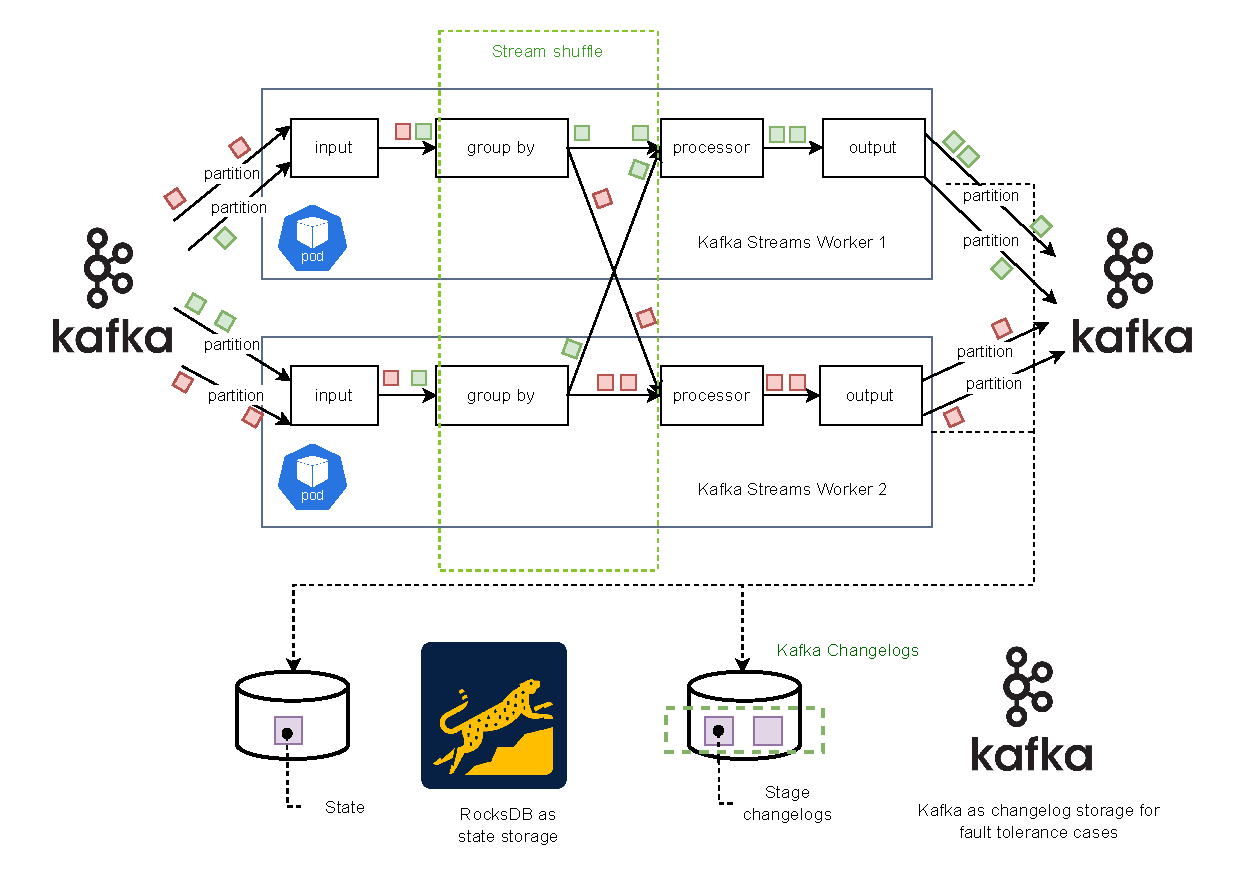
\includegraphics[width=1\textwidth]{figures/kafka/kafka-streams-workers}
    \caption{\textit{Illustrative example of Kafka Streams workers for stateful stream processing.
    implemented model also includes record match service between input and grouping blocks.}}
    \label{fig:kafka-streams-workers-general}
\end{figure}

The model on Figure \ref{fig:kafka-streams-workers-general} shows fault tolerance model which is used for
experiments with Kafka Streams.
Each Kafka Streams worker has its own local state.
In case of a fault tolerance, the state gets restored using a Kafka changelog topic.
Kafka Streams workers are intended to run only with Kafka cluster.

\newpage
\subsection{Analyzing 2-Pod Failures in an 8-Pod Cluster}\label{subsec:analyzing-2-pod-failures-in-an-8-pod-cluster}

\begin{figure}[H]
    \centering
    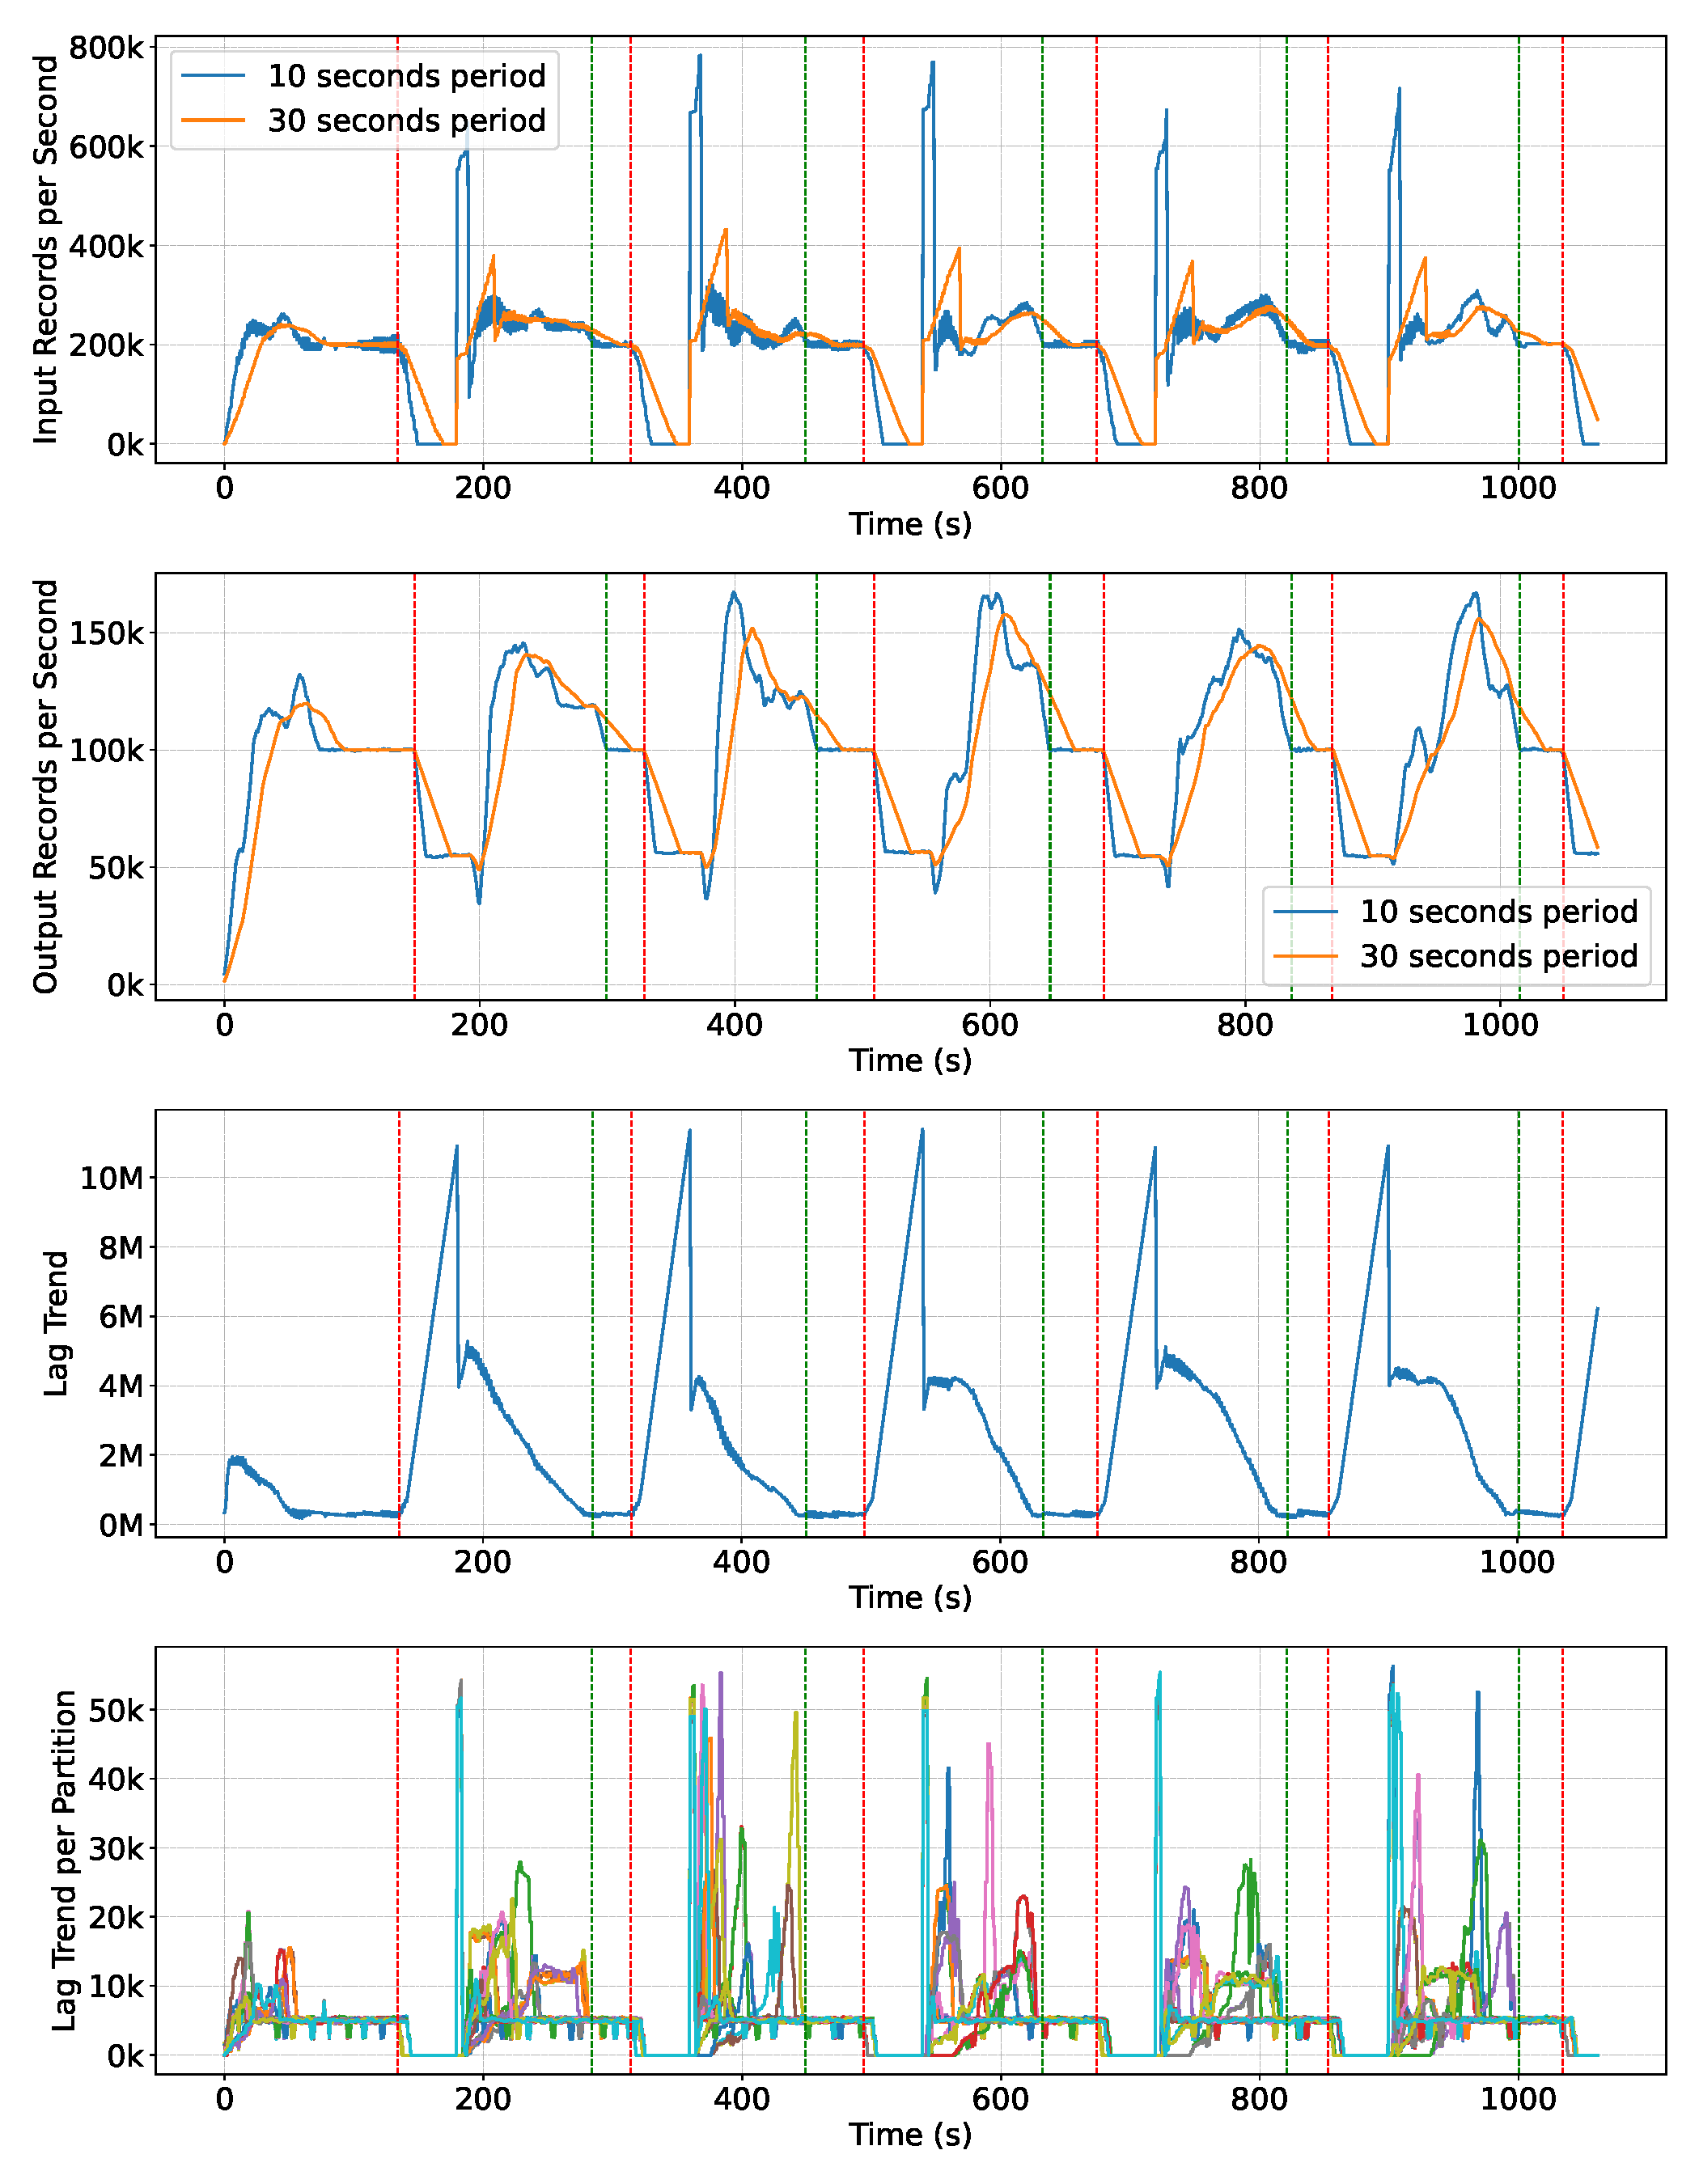
\includegraphics[width=1\textwidth]{figures/kstreams-2pods/kafka_2_pods_plot_impact}
    \caption{\textit{Benchmarks for Kafka Streams experiment in case of 2 workers failure.
    Red vertical line is a start of the failure green vertical line is a moment when the system is back to a normal state and
    producing expected load of records.}}
    \label{fig:kafka-2pods-impact}
\end{figure}

This set of benchmarks on Figure \ref{fig:kafka-2pods-impact} contains four different
benchmarks which describe system behavior for several repetitive failures.\\
The fault tolerance process based on benchmarks could be described in the following way.

\begin{description}
    \item[Workers consumer group gets stopped] \\
    During the failure, the input load and output load get stopped for a short period of time.
    At this moment, the consumer group is busy with rebalancing cluster workers and repartition
    Kafka input topic.
    Rebalancing process also includes state recalculation based on last commited records.
    \item[Consumer group lag increasing] While a consumer group is not polling new records,
    the number of uncommited records in the input topic is actively growing.
    The input topic is still getting populated by the Load generator while the consumer group
    is being repartitioned.
    In can be seen on the Lag Trend chart.
    On the Lag Trend per Partition repartition can be seen for many partitions.
    \item[Repartition is finished] Workers in the consumer group start actively polling new records
    such that the number of records in the output topic is actively growing to process
    records that have come while the consumer group wasn't polling.
    \item[The system is getting back to normal processing state]
    The cluster of workers is able to process the previously uncommited records and new incomming
    records.
    Delayed records processing is finished once the output is at 100k records per second.
\end{description}

From the green vertical line to the next red line, the system is processing the load in the
normal state.
At the next red line, the rebalancing process repeats.
Benchmarks show that rebalacing looks relevantly identically for all recorded failures.
However, such frequent failures are not expected to happen in production.
Such a rebalancing process might look the same way in case of cluster worker redeployment with a new
worker version which is working under a high load.
The process is also known as draining or draining in Kubernetes \cite{kubernetes_intro}.

Another set of benchmarks on Figure \ref{fig:kafka-2pods-resource} show consumed resources for all workers during the experiment.
These benchmarks show how a network traffic and CPU utilization change during a state recovery.
Network traffic keeps being stable while the system is in a normal processing state.
The average time from a fault to a normal execution state is about 143 seconds.


\begin{figure}[H]
    \centering
    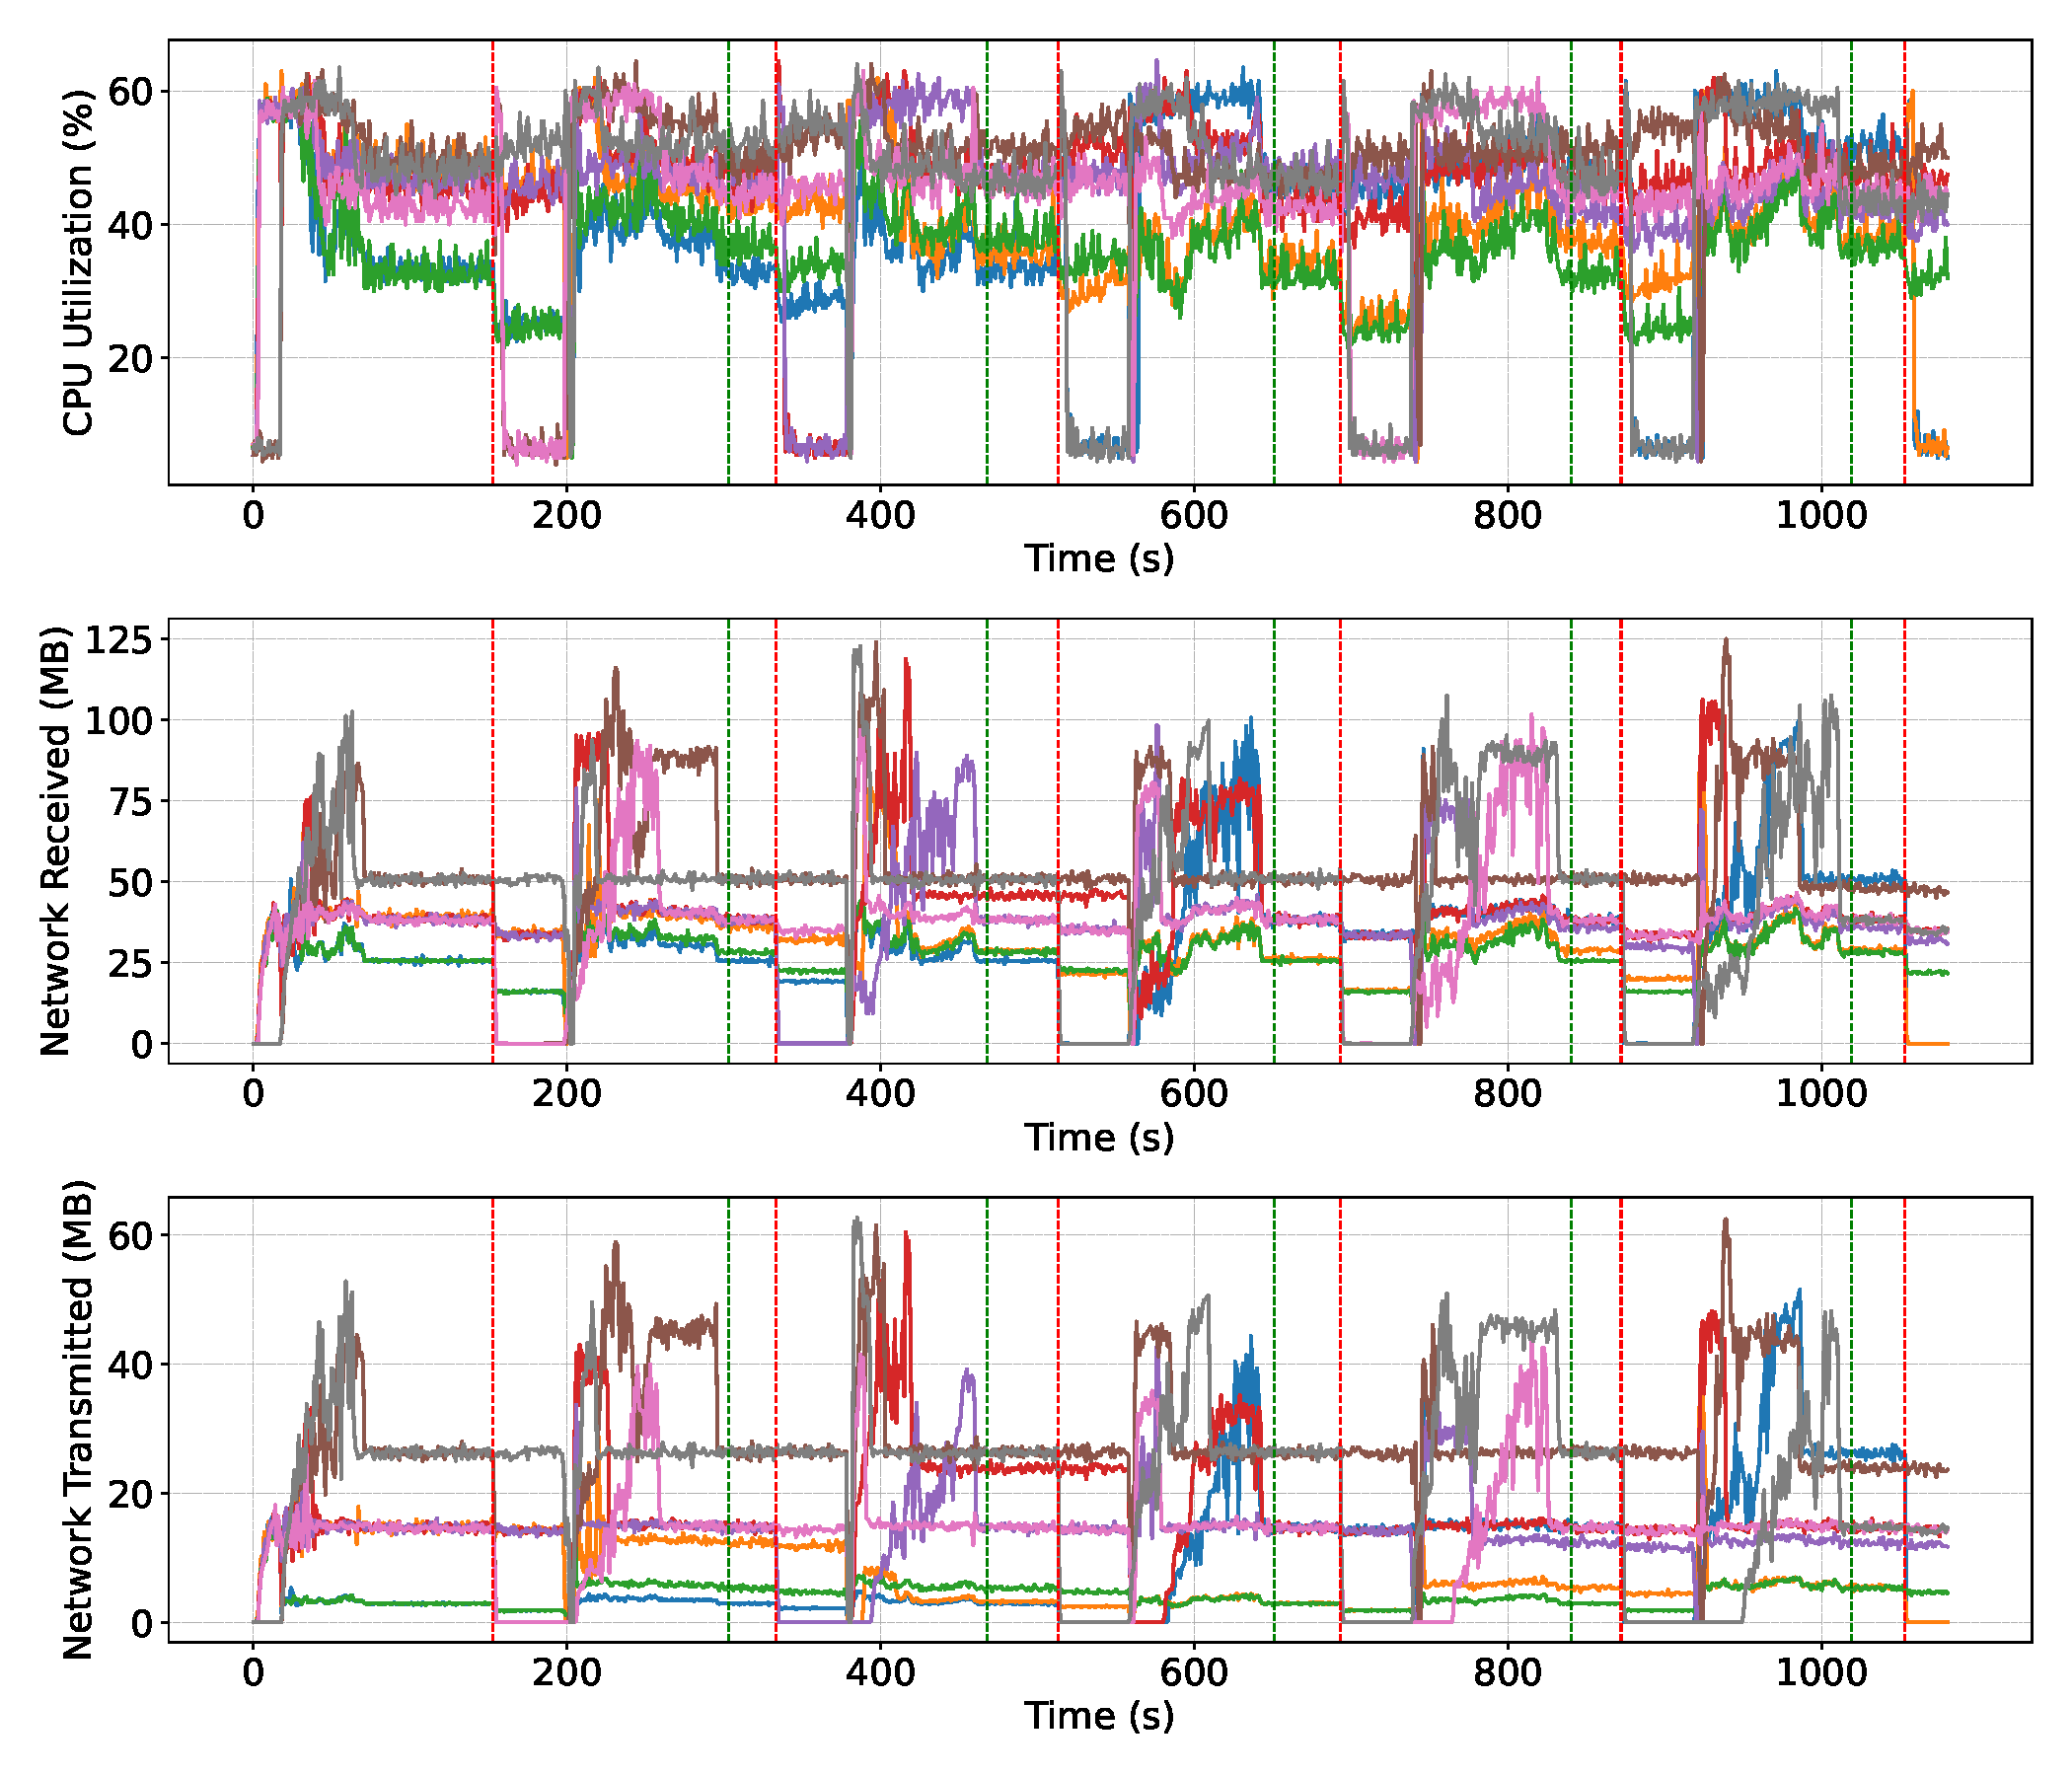
\includegraphics[width=1\textwidth]{figures/kstreams-2pods/kafka_2_pods_resources}
    \caption{\textit{Resources consumption during a state recovery in case of 2 worker failures.}}
    \label{fig:kafka-2pods-resource}
\end{figure}


\newpage
\subsection{Analyzing 8-Pod Failures in an 8-Pod Cluster}\label{subsec:analyzing-8-pod-failures-in-an-8-pod-cluster}

\begin{figure}[H]
    \centering
    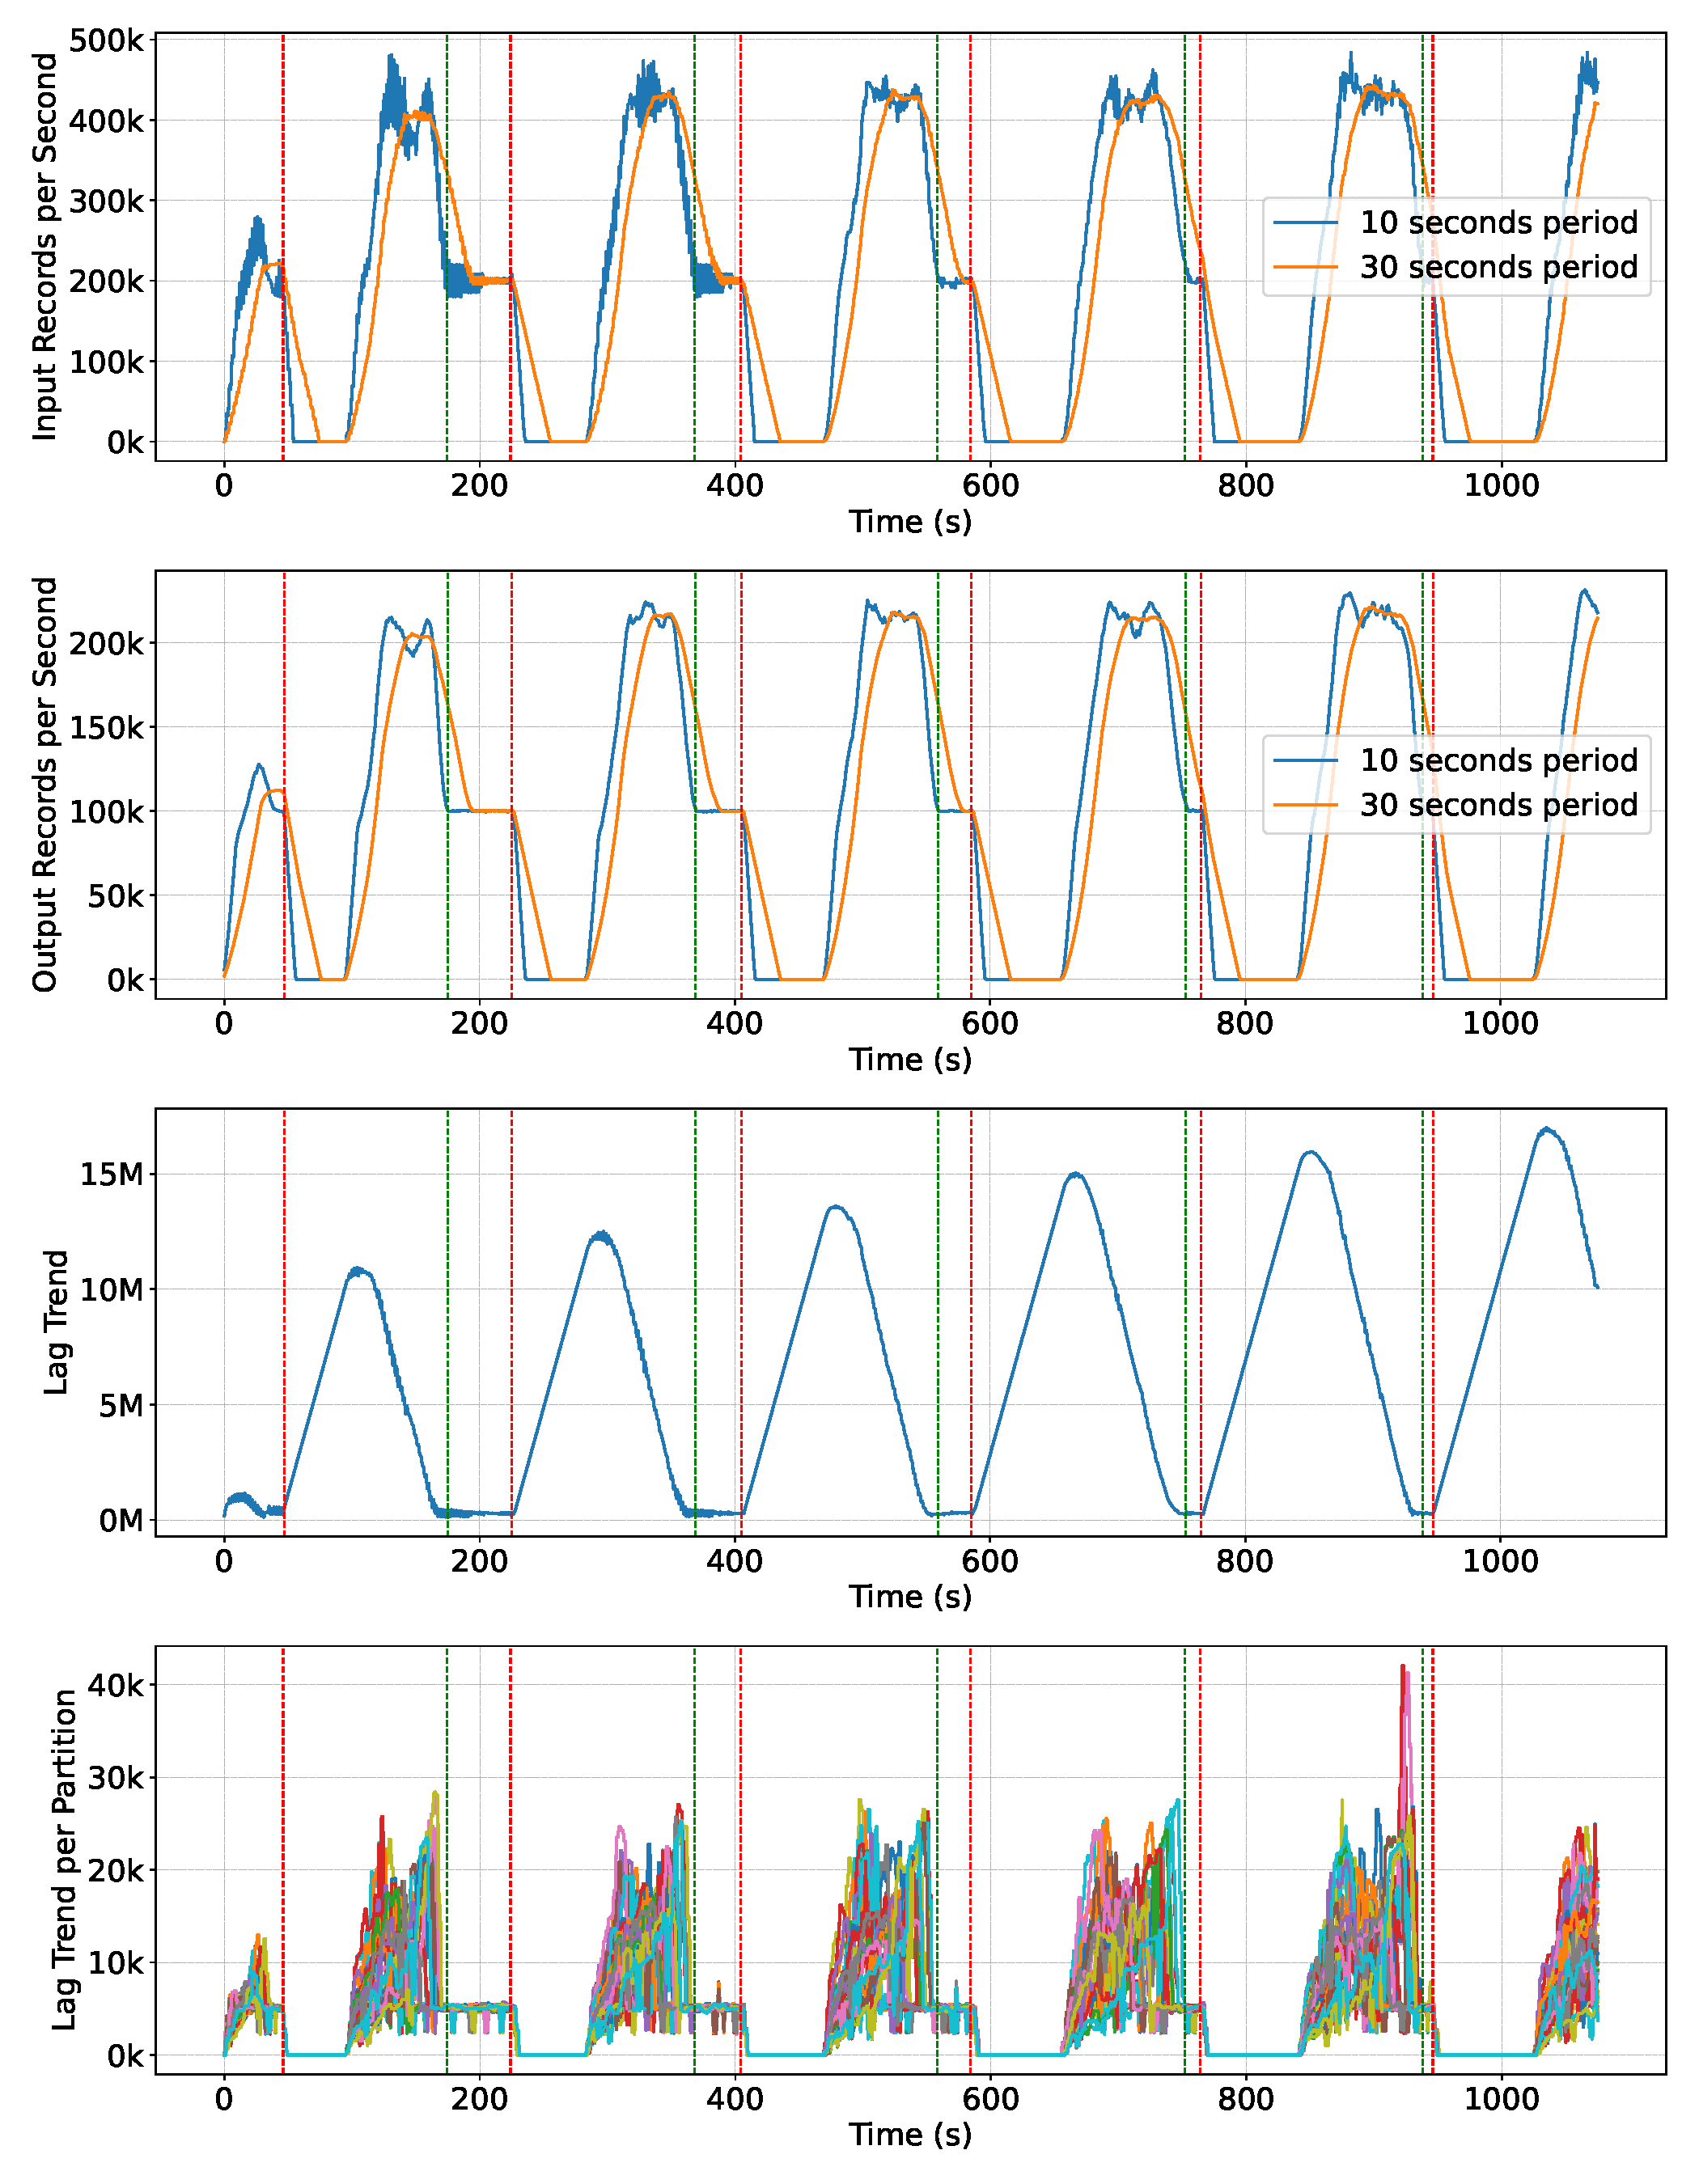
\includegraphics[width=1\textwidth]{figures/kstreams-8pods/kafka_8_pods_plot_impact}
    \caption{\textit{Benchmarks for Kafka Streams experiment in case of 8 workers failure.
    Worker cluster is fully killed. Red vertical line is a start of the failure green vertical line is a moment when the system is back
to a normal state and producing expected load of records.}}
    \label{fig:kafka-8pods-impact}
\end{figure}

This experiment is trying to get metrics for the case when all workers get killed.
It has the same rebalacing life cycle as described in the first experiment. \ref{subsec:analyzing-2-pod-failures-in-an-8-pod-cluster}
According to benchmarks on Figure \ref{fig:kafka-8pods-impact} The average time from a fault to a normal execution state is about 153 seconds,
that is only 10 seconds longer than in experiment \ref{subsec:analyzing-2-pod-failures-in-an-8-pod-cluster}.
However, network resources consumption is more extensive since all workers are involved Figure \ref{fig:kafka-8pods-resource}.
Also, all partitions are involved into repartition, which can be seen on Figure \ref{fig:kafka-8pods-impact}
for Lag Trend and Lag Trend per Partition.


\begin{figure}[ht]
    \centering
    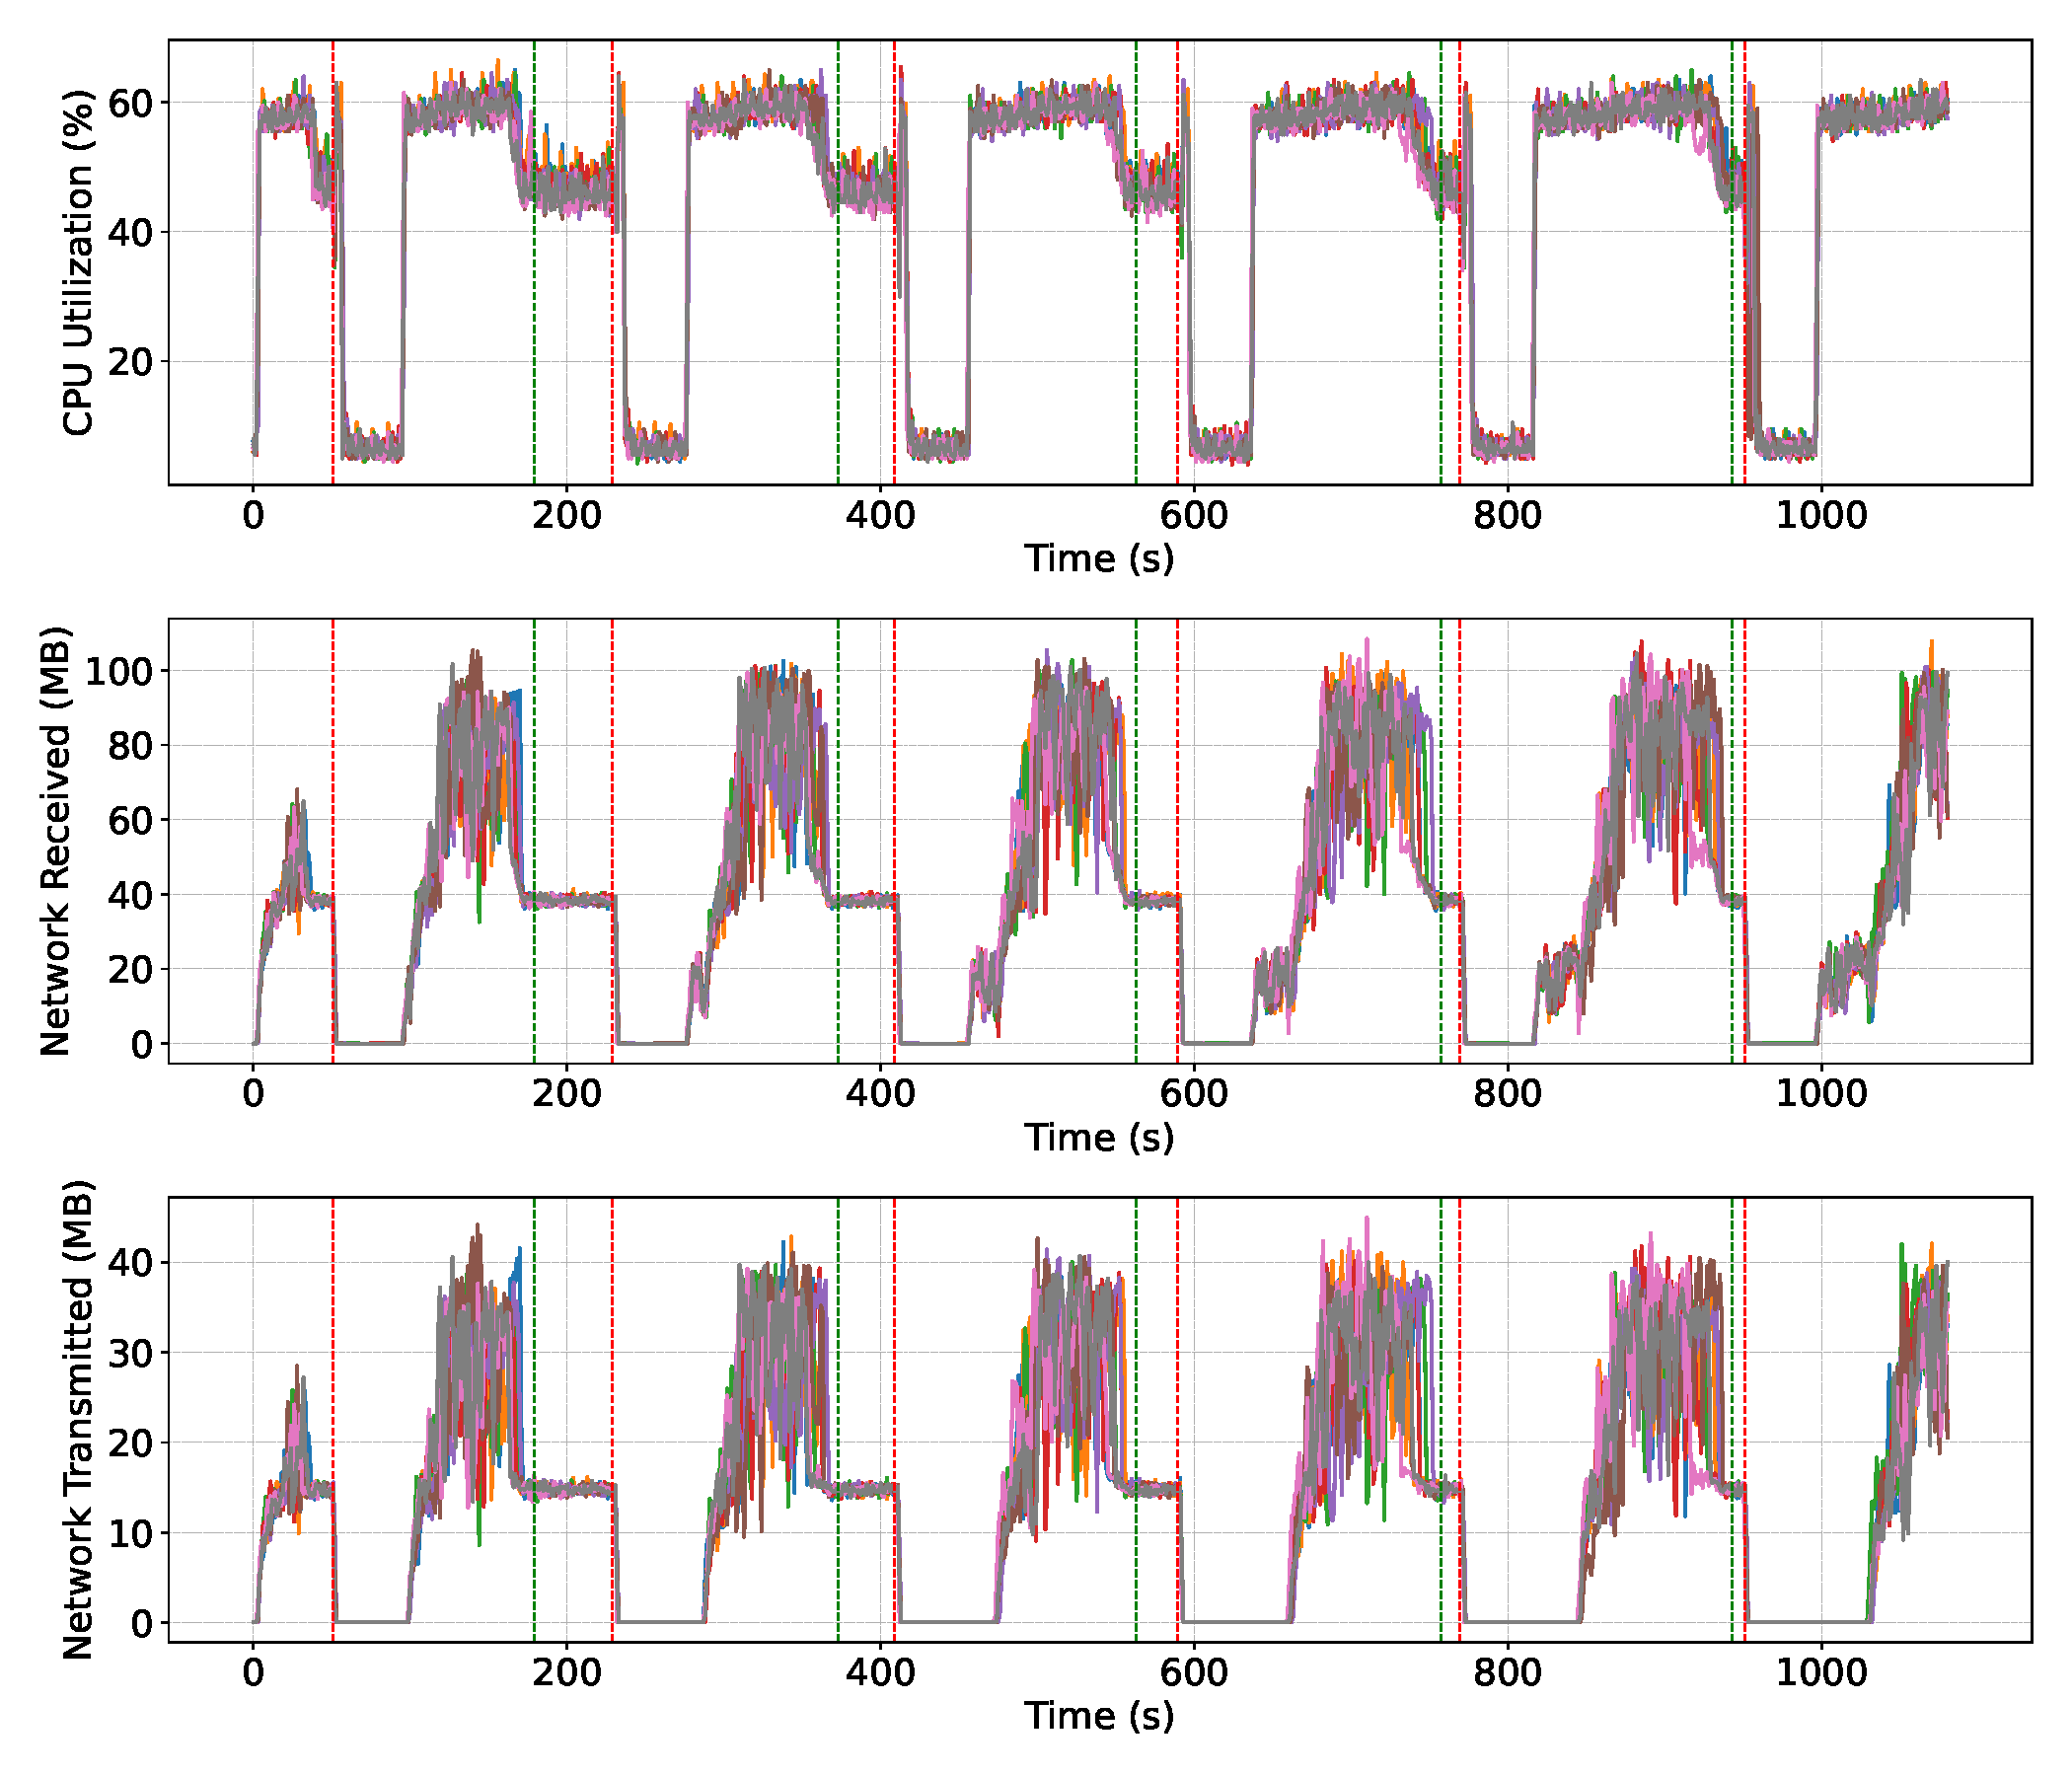
\includegraphics[width=1\textwidth]{figures/kstreams-8pods/kafka_8_pods_resources}
    \caption{\textit{Resources consumption during a state recovery in case of 8 worker failures in a cluster of 8 workers.}}
    \label{fig:kafka-8pods-resource}
\end{figure}



\newpage
\section{Benchmarking Apache Flink Fault Tolerance}\label{sec:benchmarking-apache-flink-fault-tolerance}

\begin{figure}[H]
    \centering
    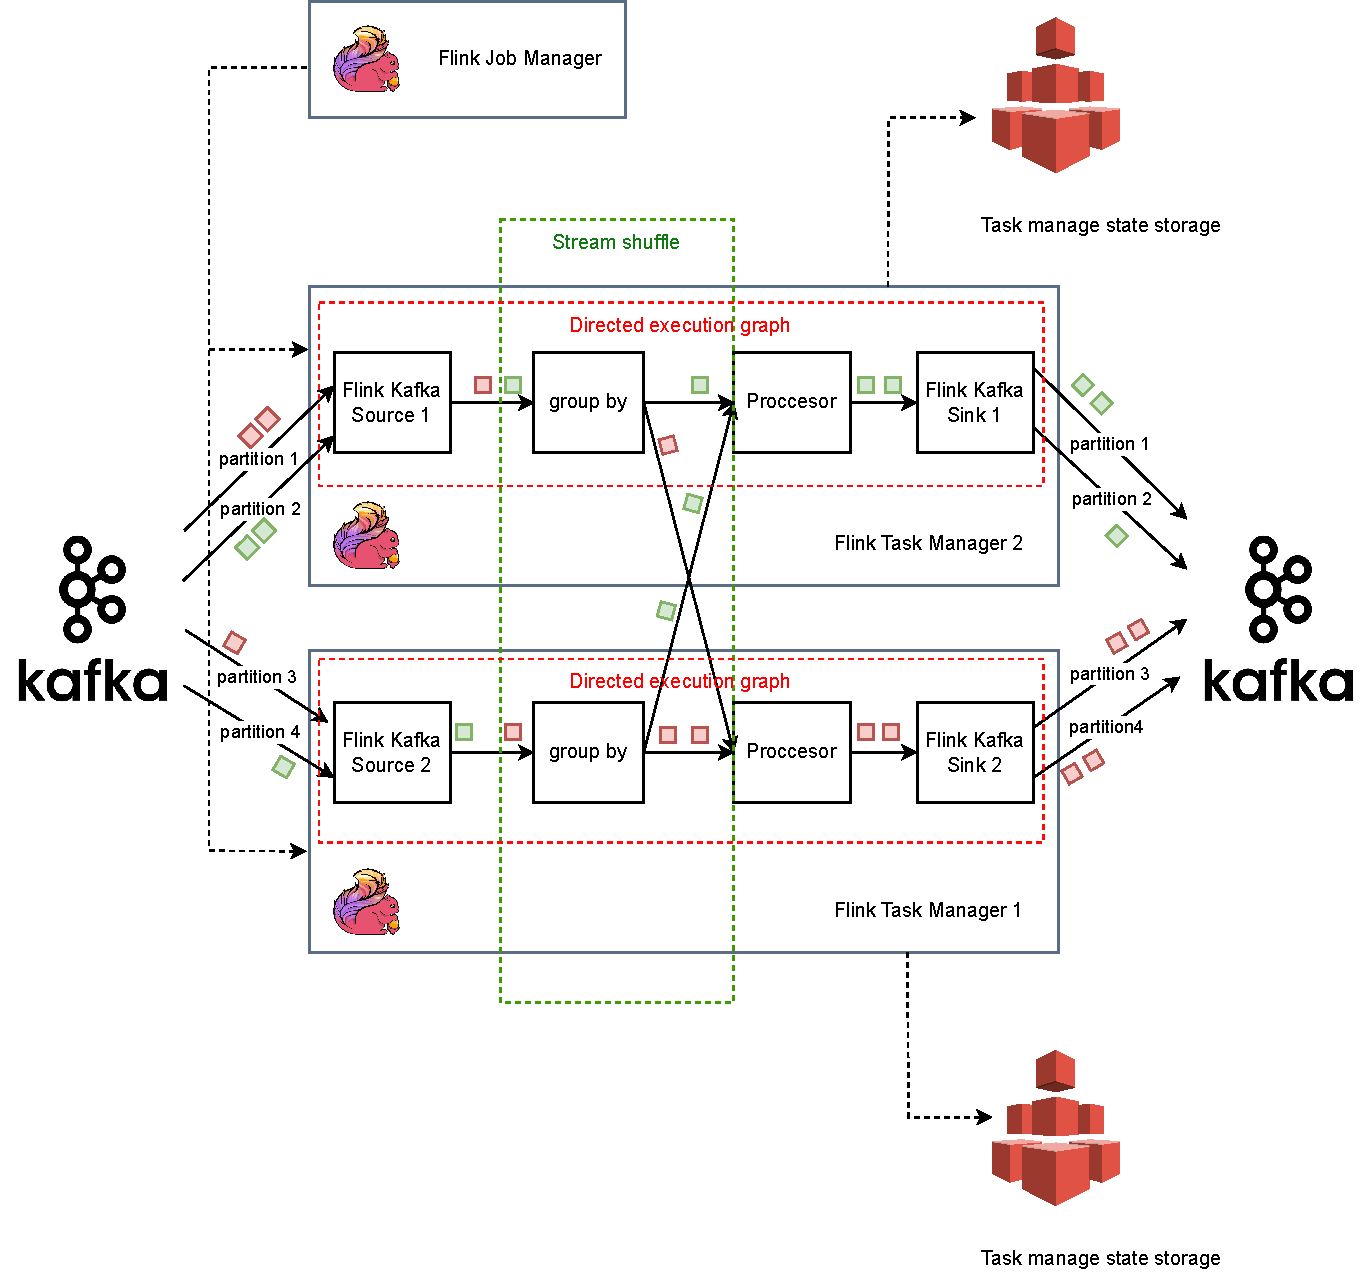
\includegraphics[width=1\textwidth]{figures/flink/flink-shuffle-workers}
    \caption{\textit{Illustrative example of Apache Flink workers for stateful stream processing.
    implemented prototype also includes record match service between input and grouping blocks.}}
    \label{fig:flink-workers-general}
\end{figure}

The prototype model on Figure \ref{fig:flink-workers-general} is based on Apache Flink.
It uses the same Kafka input and Kafka output topics as Kafka Streams prototype on Figure \ref{fig:kafka-streams-workers-general}.
Important difference for Kafka Streams implementation is that Flink uses checkpoints for
state recovery.
In this prototype, the state checkpoints are stored in EFS network storage which is mounted and connected to
Flink workers using Kubernetes and AWS storage configuration.


\subsection{Analyzing 2-Pod Failures in an 8-Pod Cluster}\label{subsec:analyzing-2-pod-failures-in-an-8-pod-cluster2}

\begin{figure}[H]
    \centering
    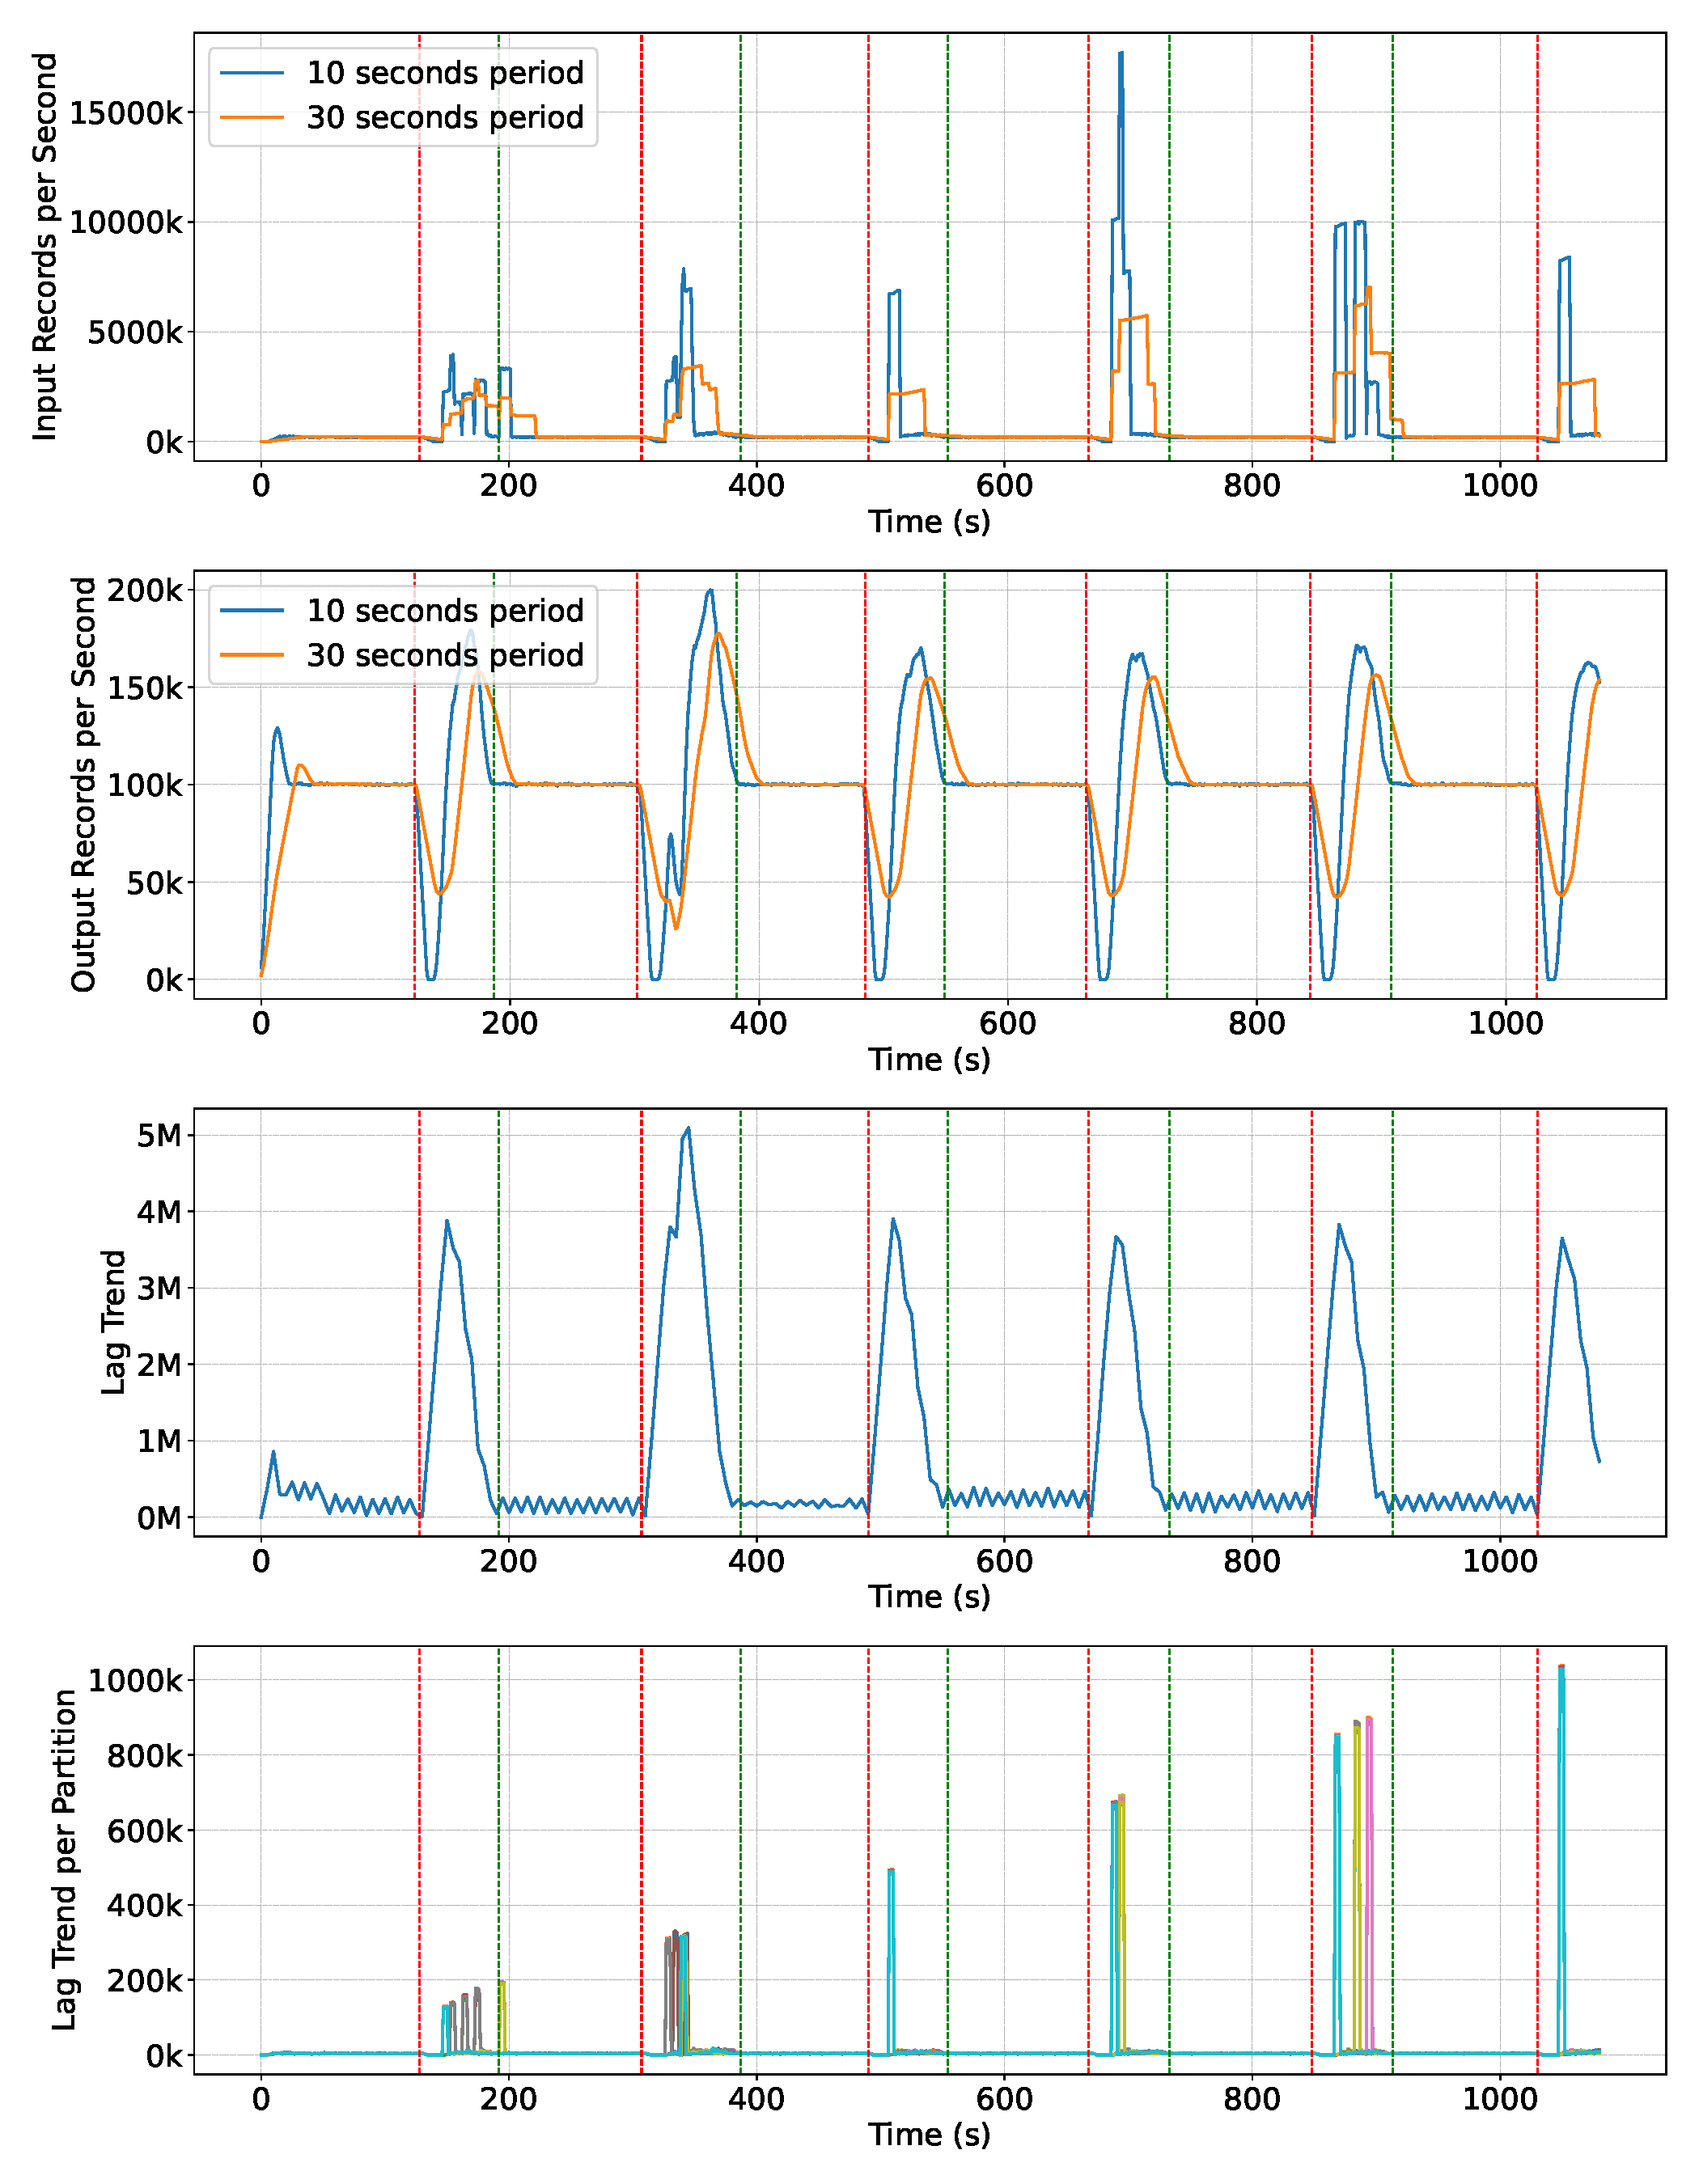
\includegraphics[width=1\textwidth]{figures/flink-2pods/flink_2_pods_plot_impact}
    \caption{\textit{Benchmarks for Apache Flink experiment in case of 2 workers failure. Worker
cluster is fully killed. Red vertical line is a start of the failure green vertical line is a
moment when the system is back to a normal state and producing expected load of records.}}
    \label{fig:flink-2pods-impact}
\end{figure}

Balancing process is also the same as described in \ref{subsec:analyzing-2-pod-failures-in-an-8-pod-cluster},
Since Flink worker cluster is also a Kafka consumer group that's polling records from a Kafka input topic.
On the Figure \ref{fig:flink-2pods-impact} depicted the same benchmarks as on Figure \ref{fig:kafka-2pods-impact}.
Benchmarks on Figure \ref{fig:flink-2pods-resource} denote resource consumption.
The average time from a fault to a normal execution state is about 113 seconds.

\begin{figure}[ht]
    \centering
    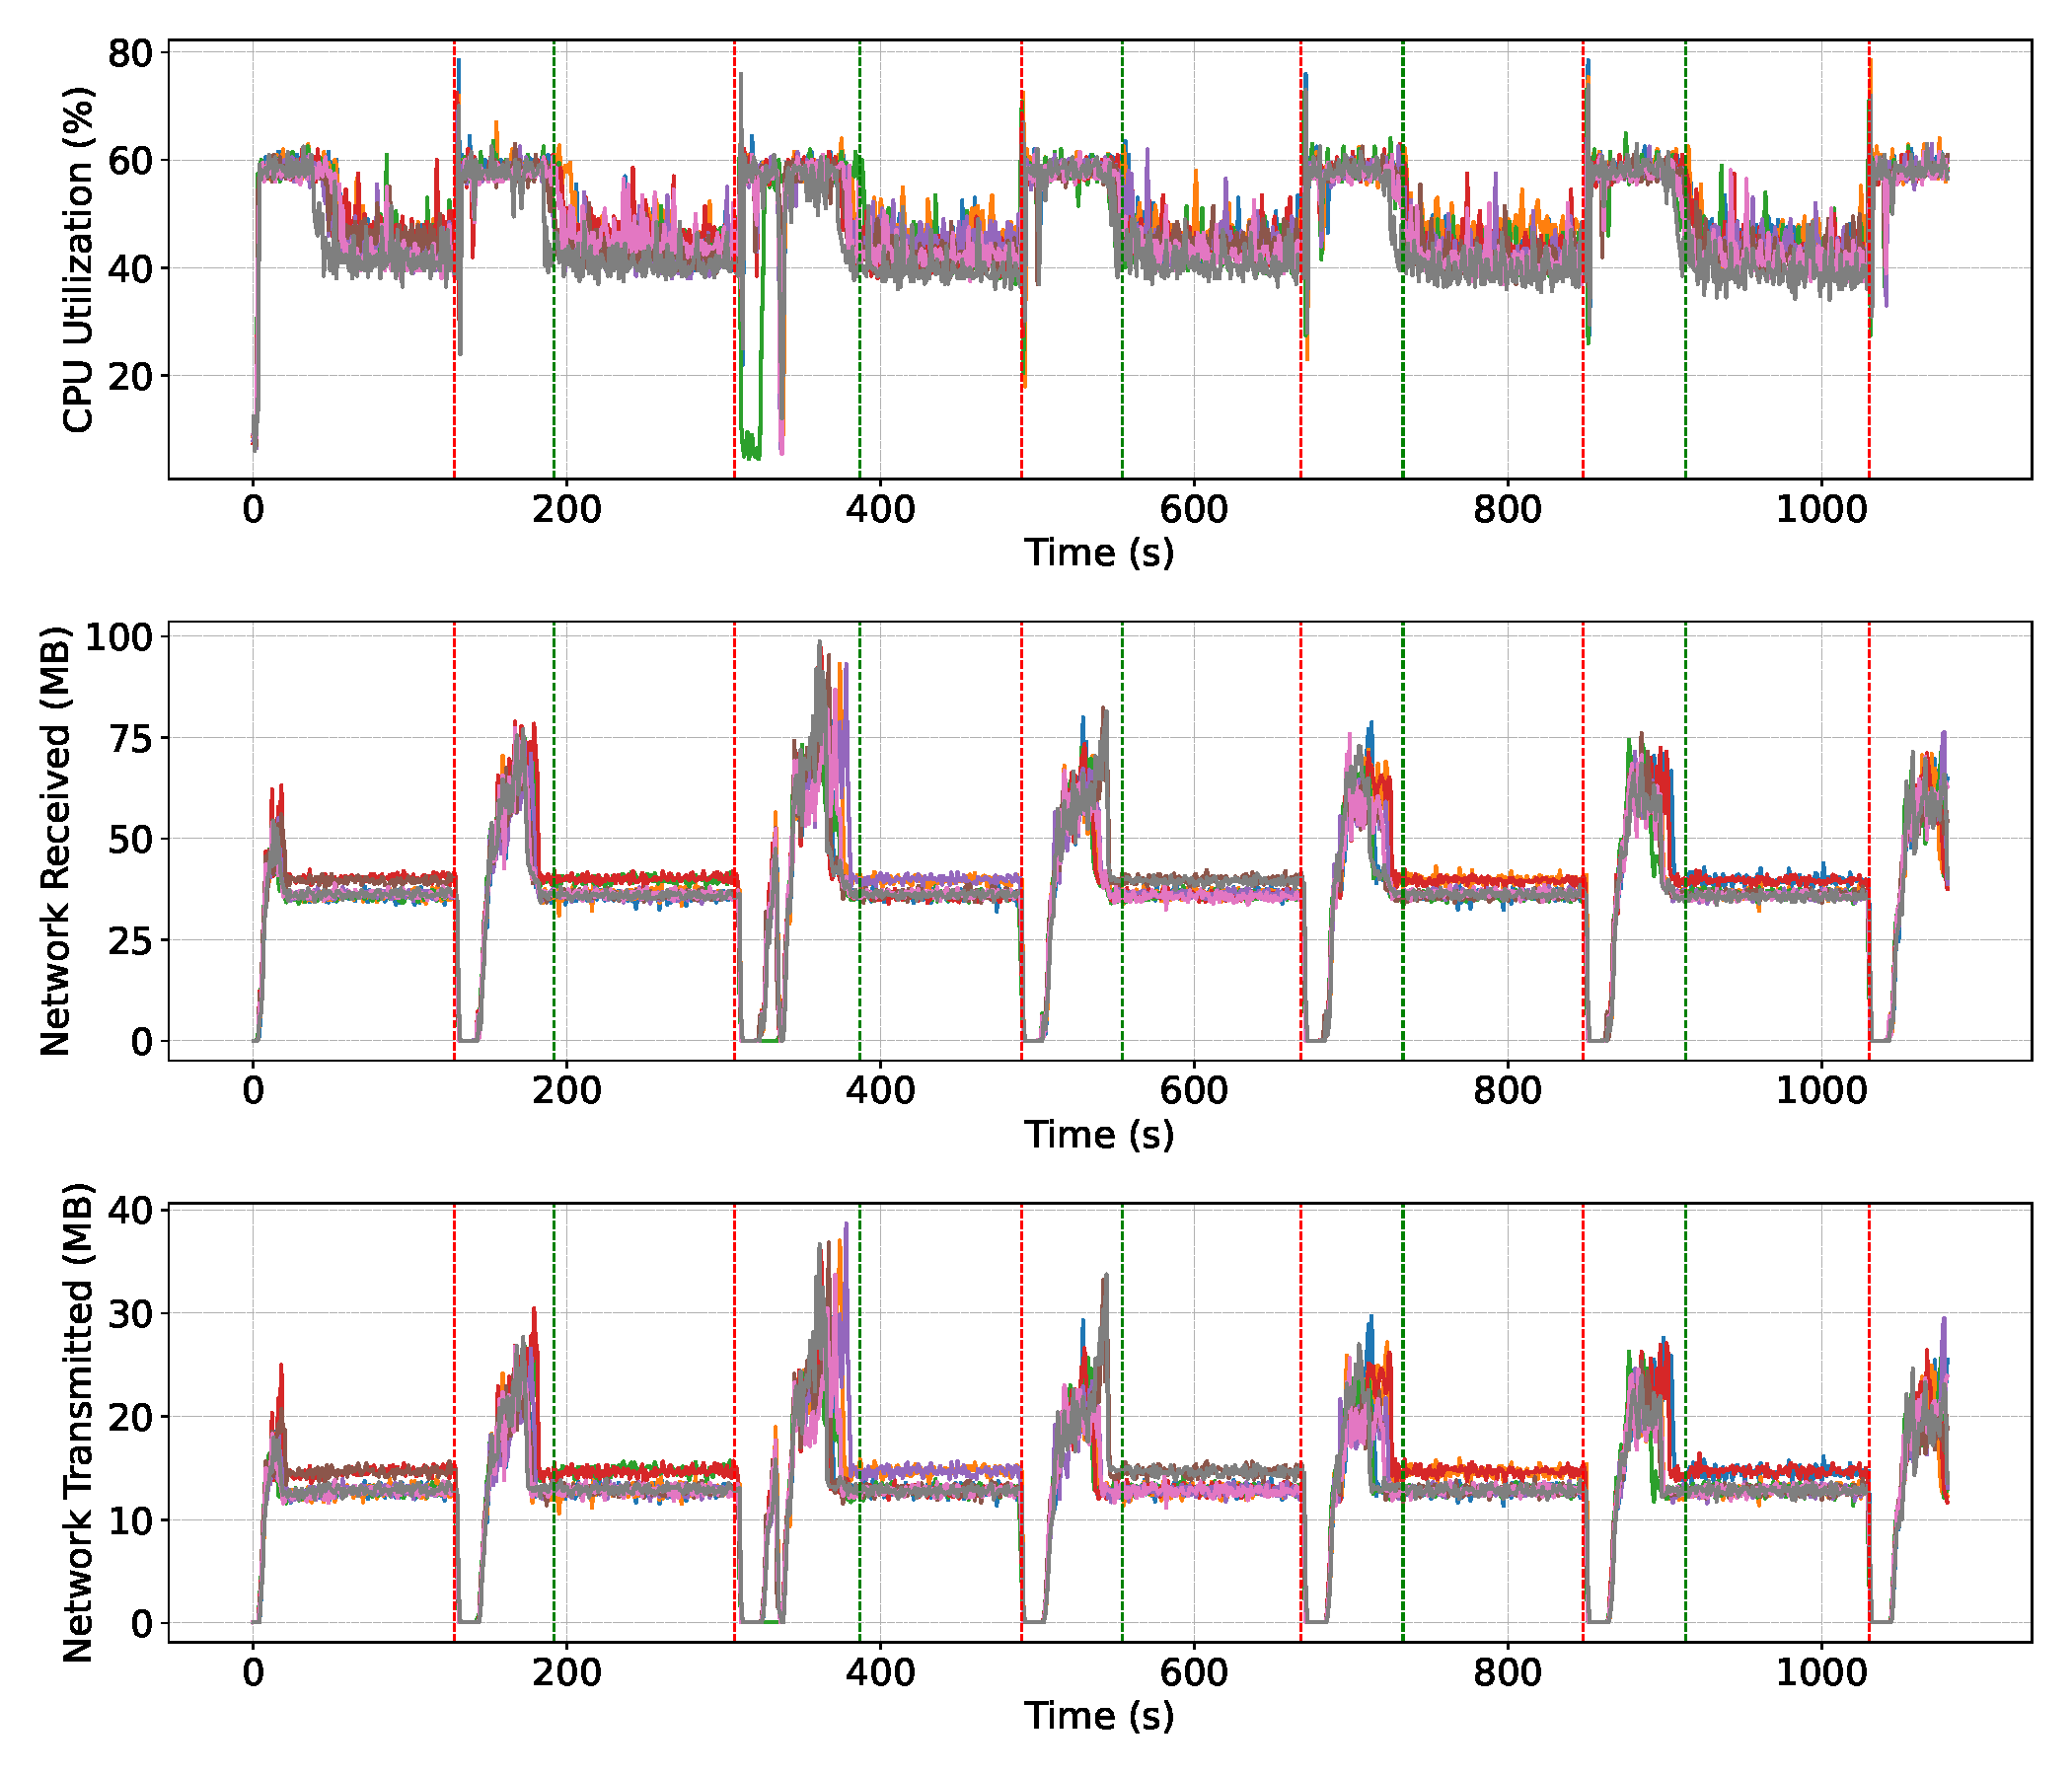
\includegraphics[width=1\textwidth]{figures/flink-2pods/flink_2_pods_resources}
    \caption{\textit{Resources consumption during a state recovery in case of 2 worker failures.}}
    \label{fig:flink-2pods-resource}
\end{figure}


\newpage
\subsection{Analyzing 8-Pod Failures in an 8-Pod Cluster}\label{subsec:analyzing-8-pod-failures-in-an-8-pod-cluster2}

\begin{figure}[H]
    \centering
    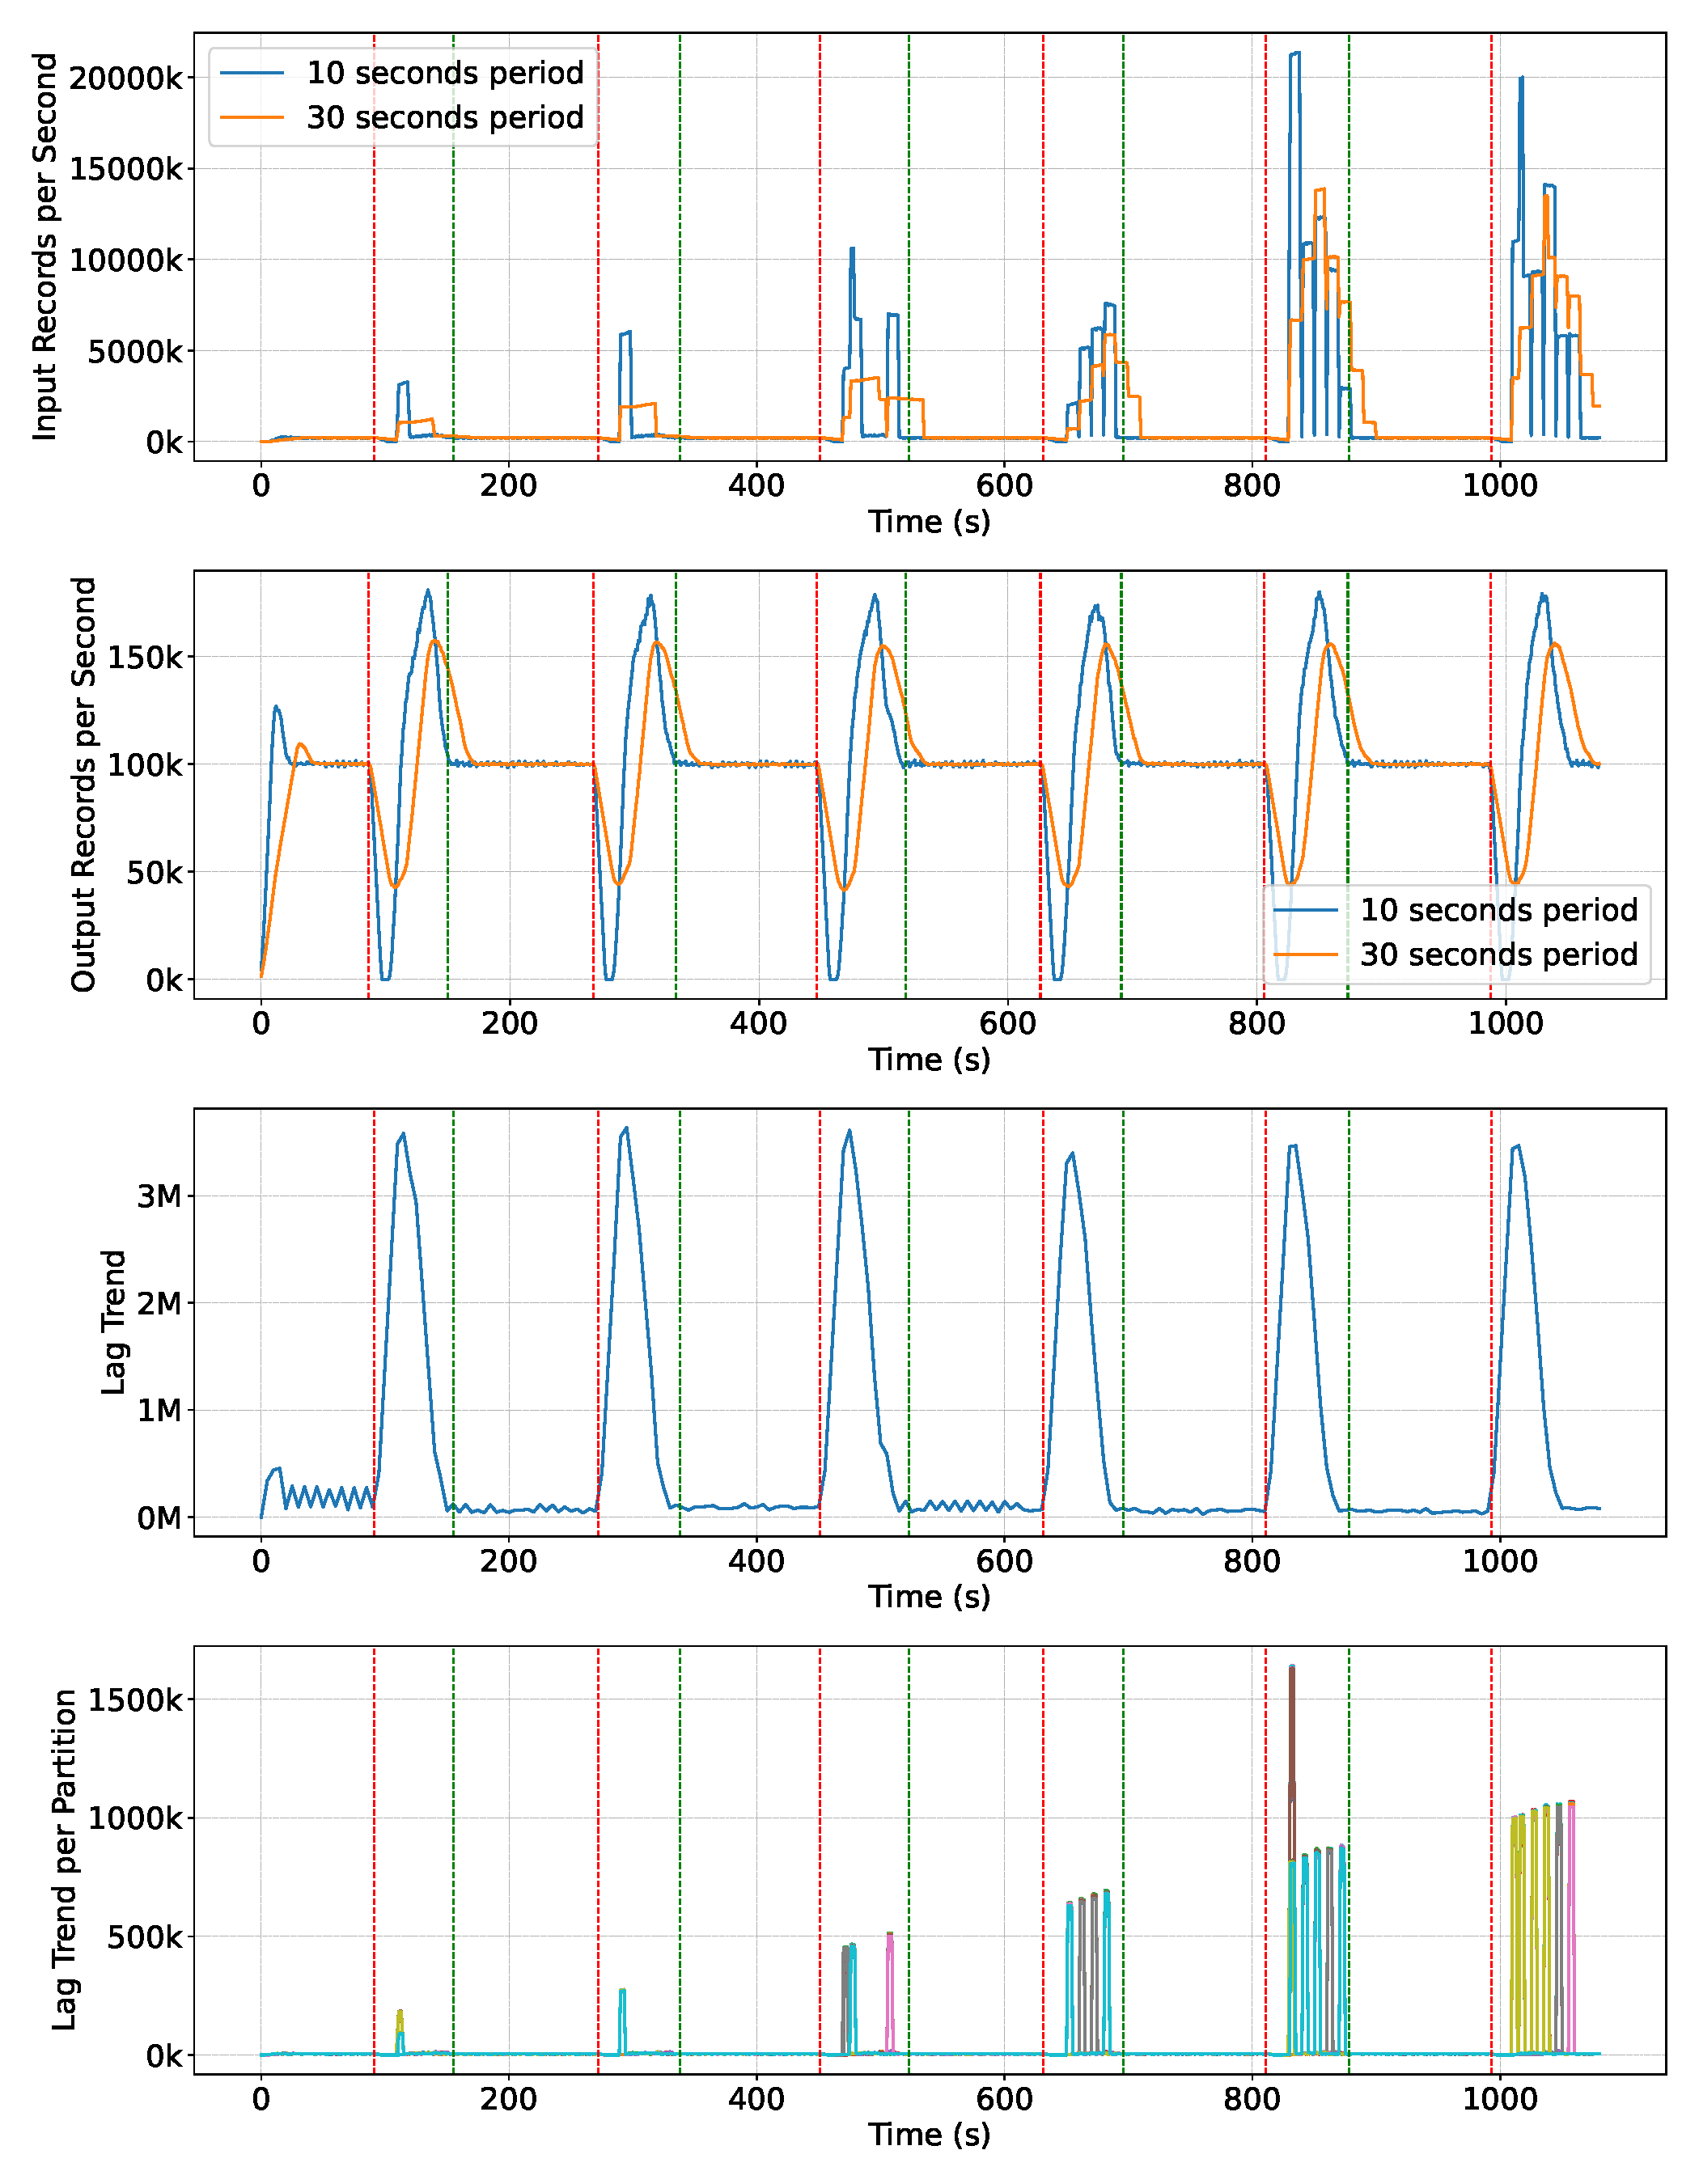
\includegraphics[width=1\textwidth]{figures/flink-8pods/flink_8_pods_plot_impact}
    \caption{\textit{Benchmarks for Apache Flink experiment in case of 8 workers failure.
    Worker cluster is fully killed. Red vertical line is a start of the failure green vertical line is a moment when the system is back
    to a normal state and producing expected load of records.}}
    \label{fig:flink-8pods-impact}
\end{figure}

These benchmarks on Figure \ref{fig:flink-8pods-impact} and resources consumption benchmarks on Figure \ref{fig:flink-8pods-resource}
denote Apache Flink performance in case of all workers in worker cluster get killed.
The average time from a fault to a normal execution state is about 114 seconds.
That it's quite an impressive result, 1 second difference comparing to benchmarks
with 2 workers on Figure \ref{fig:flink-2pods-impact}.


\begin{figure}[H]
    \centering
    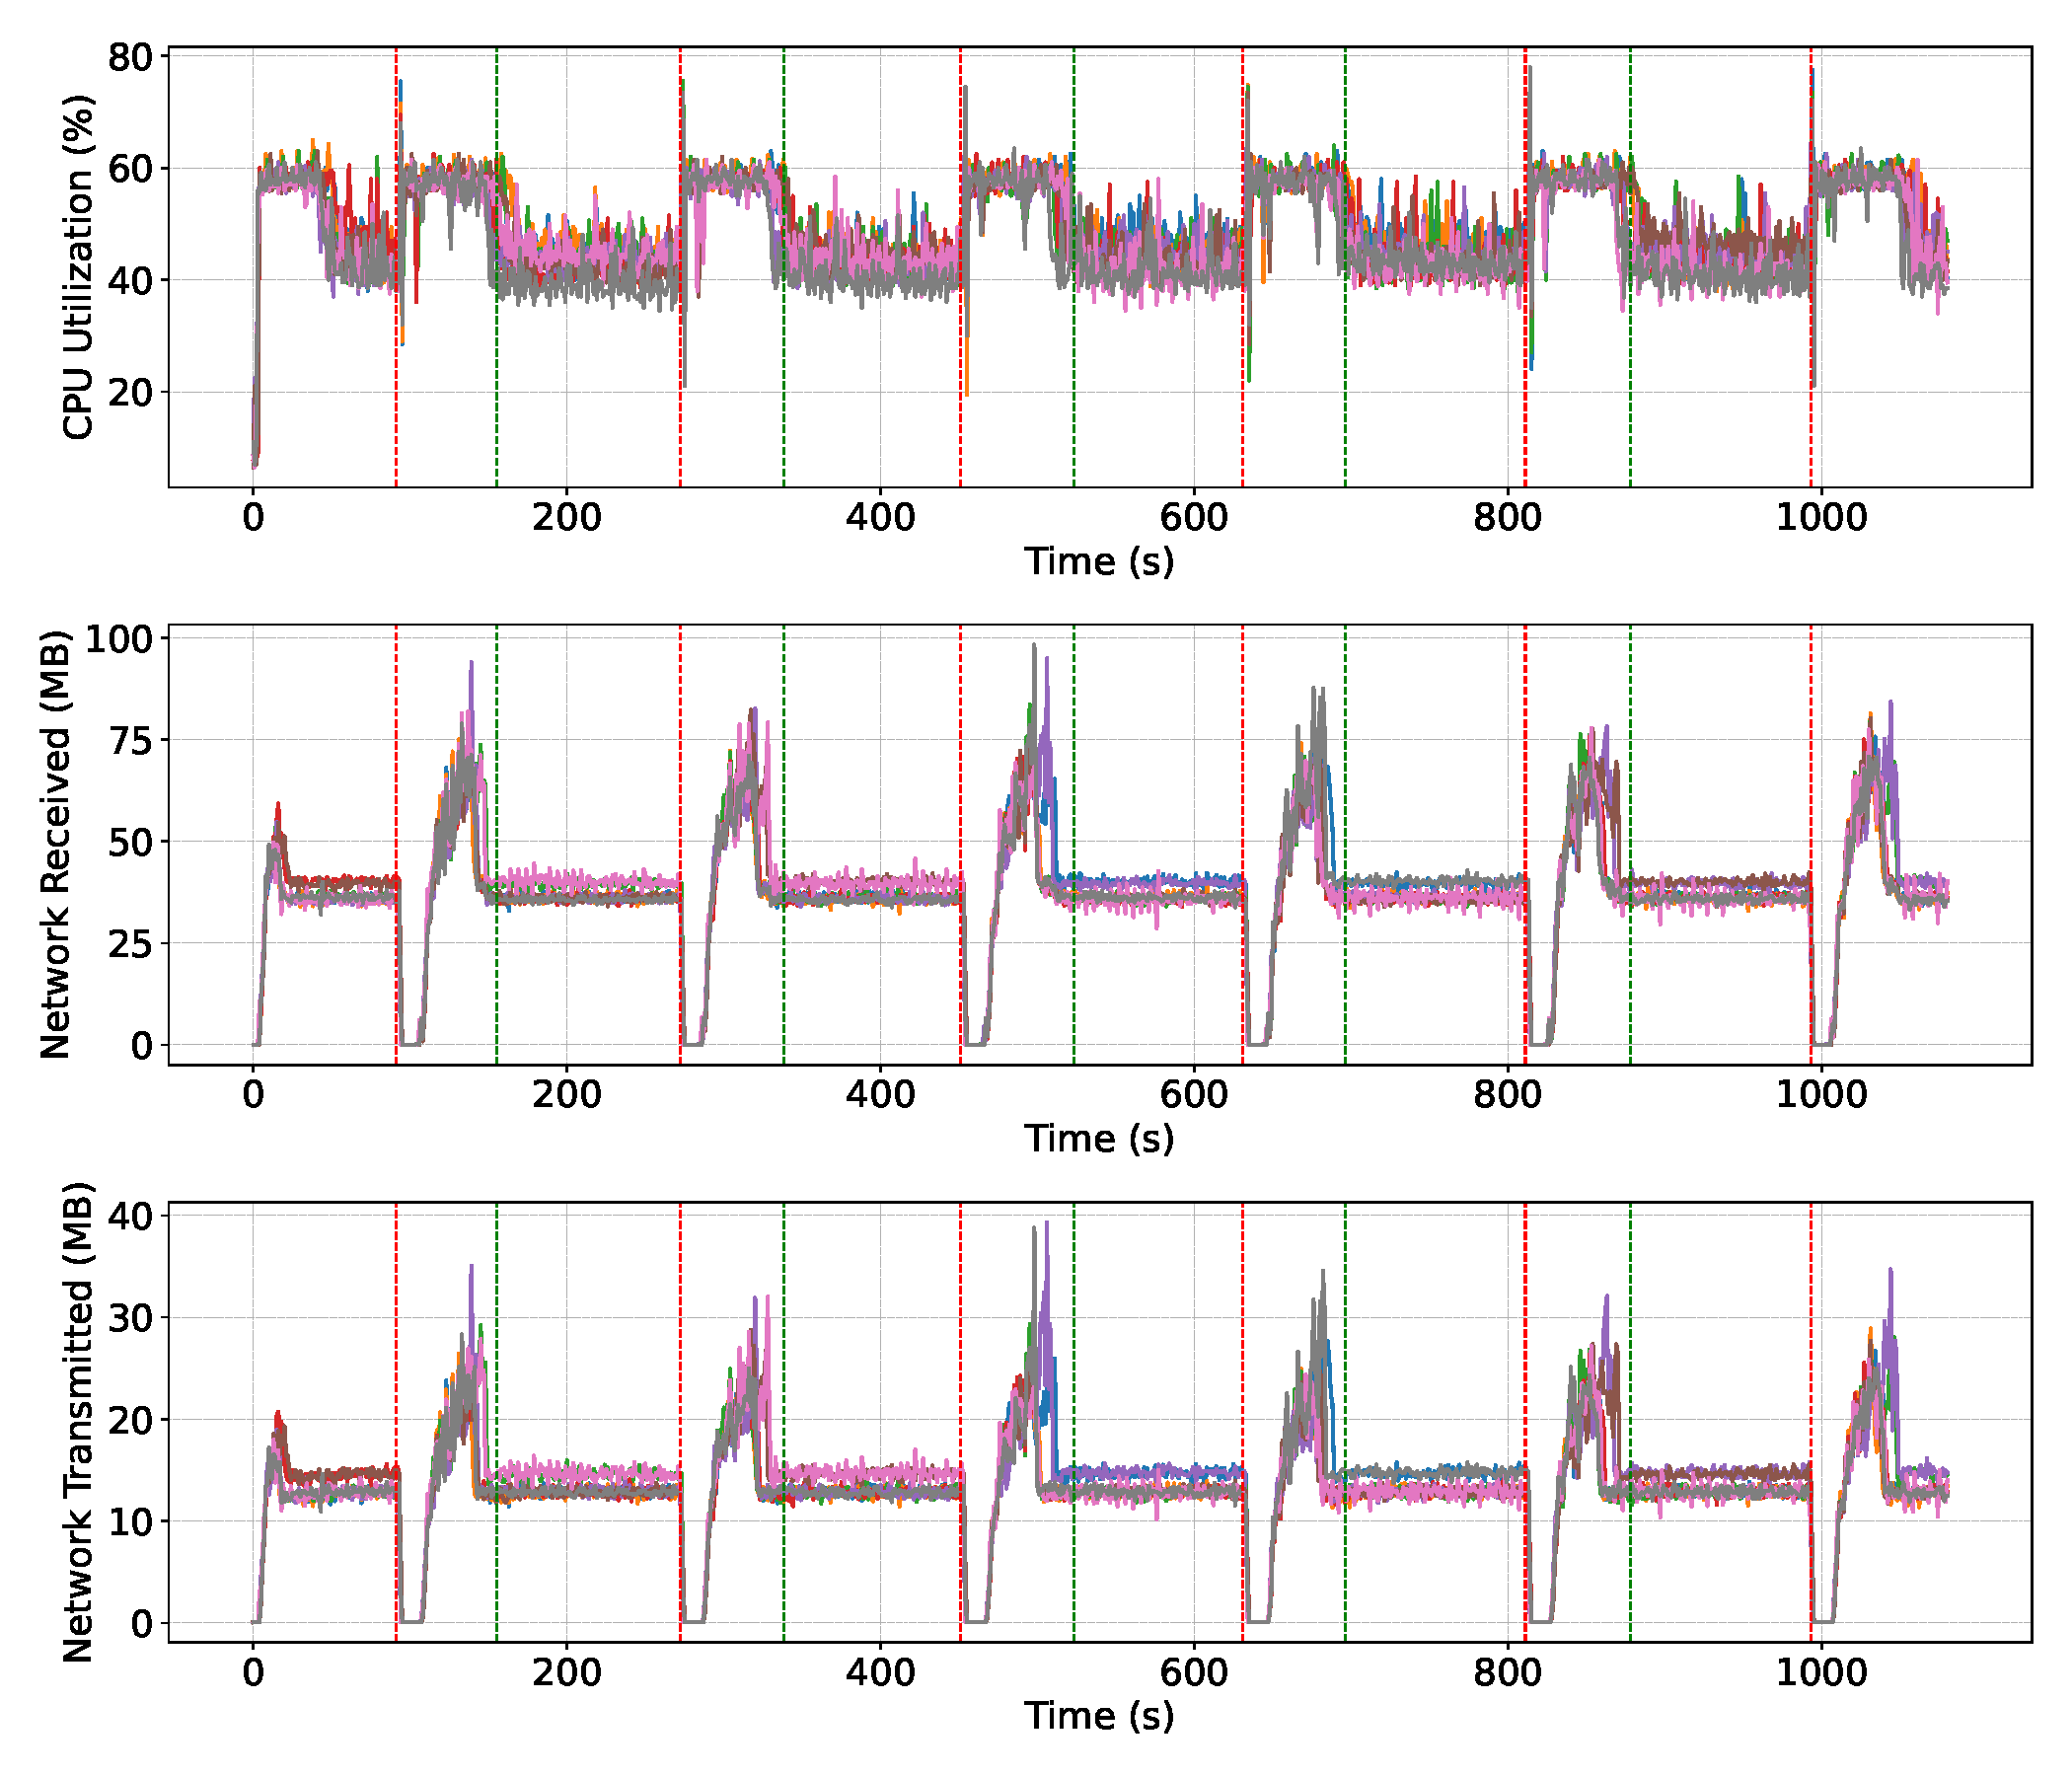
\includegraphics[width=1\textwidth]{figures/flink-8pods/flink_8_pods_resources}
    \caption{\textit{Resources consumption during a state recovery in case of 8 worker failures.}}
    \label{fig:flink-8pods-resource}
\end{figure}


\newpage
\section{Comparative analysis}\label{subsec:comparative-analysis}
This section is comparing Apache Flink and Kafka Streams benchmarks
on the same chart to observe a behavior difference in two systems.
Important notice, workers failures happened in different moments since
for Kafka Streams and Flink, due to Chaos Mesh cron jobs.

\subsection{Input throughput}\label{subsec:input-throughtput}

\begin{figure}[H]
    \centering
    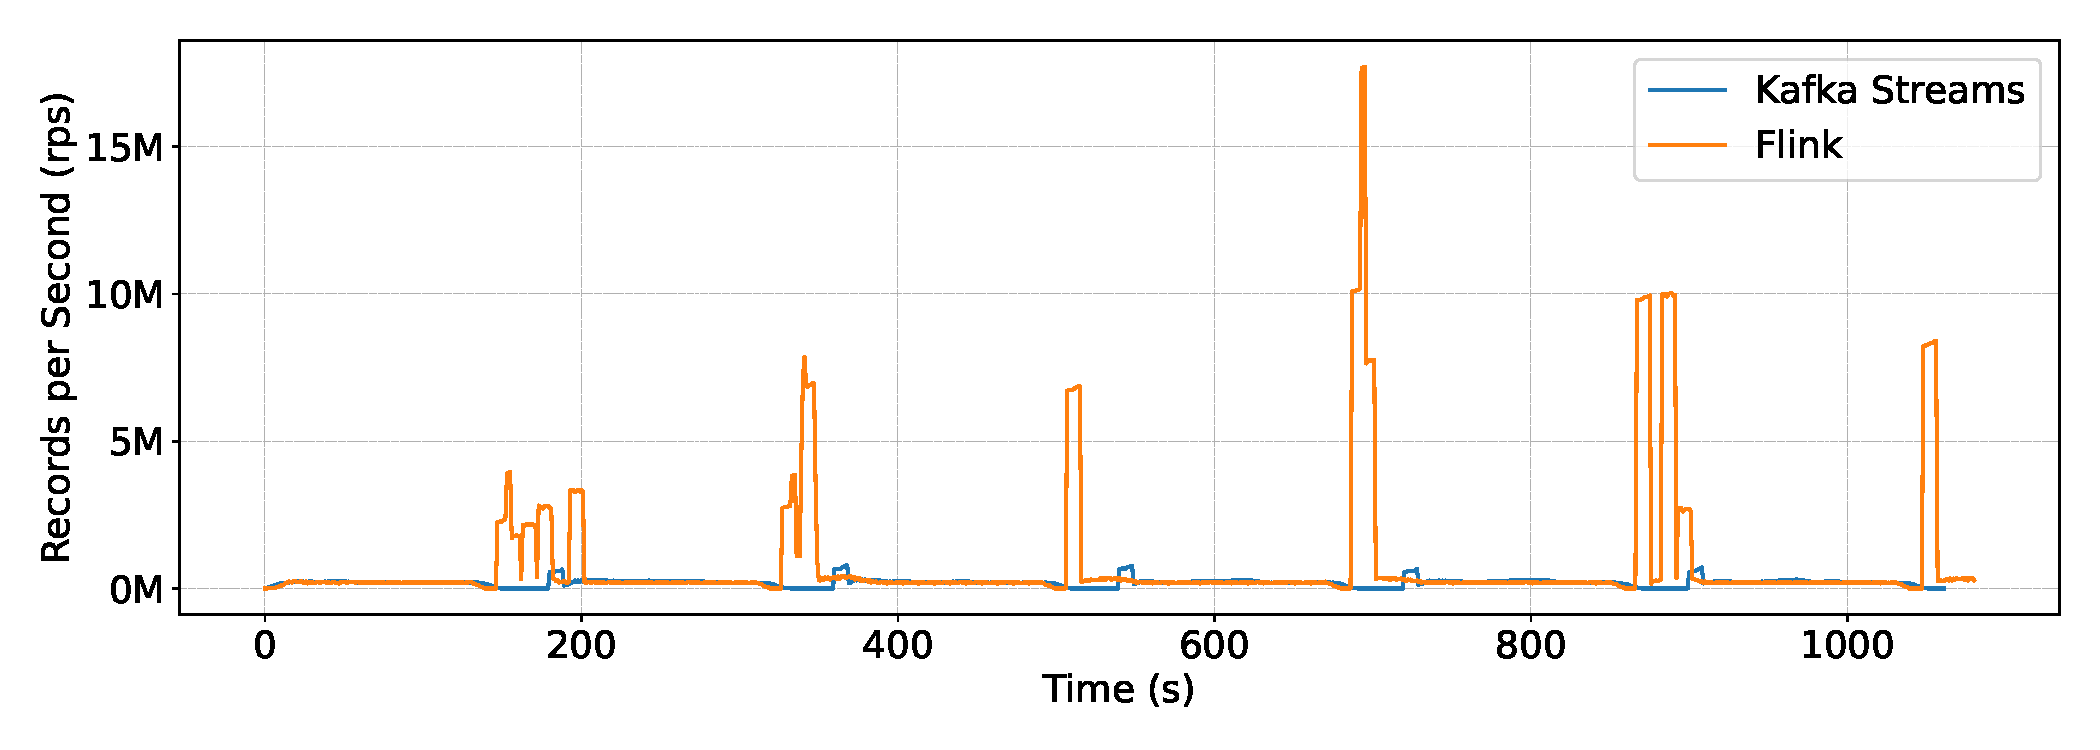
\includegraphics[width=1\textwidth]{figures/kafka-flink/input-throughput-2pod-kafka-flink}
    \caption{\textit{Input throughput for Kafka records in case of 2 workers.
    Failure period for kafka Stream and Apache Flink is not synced but happens within the same period.}}
    \label{fig:kafka-flink-input-2}
\end{figure}


\begin{figure}[H]
    \centering
    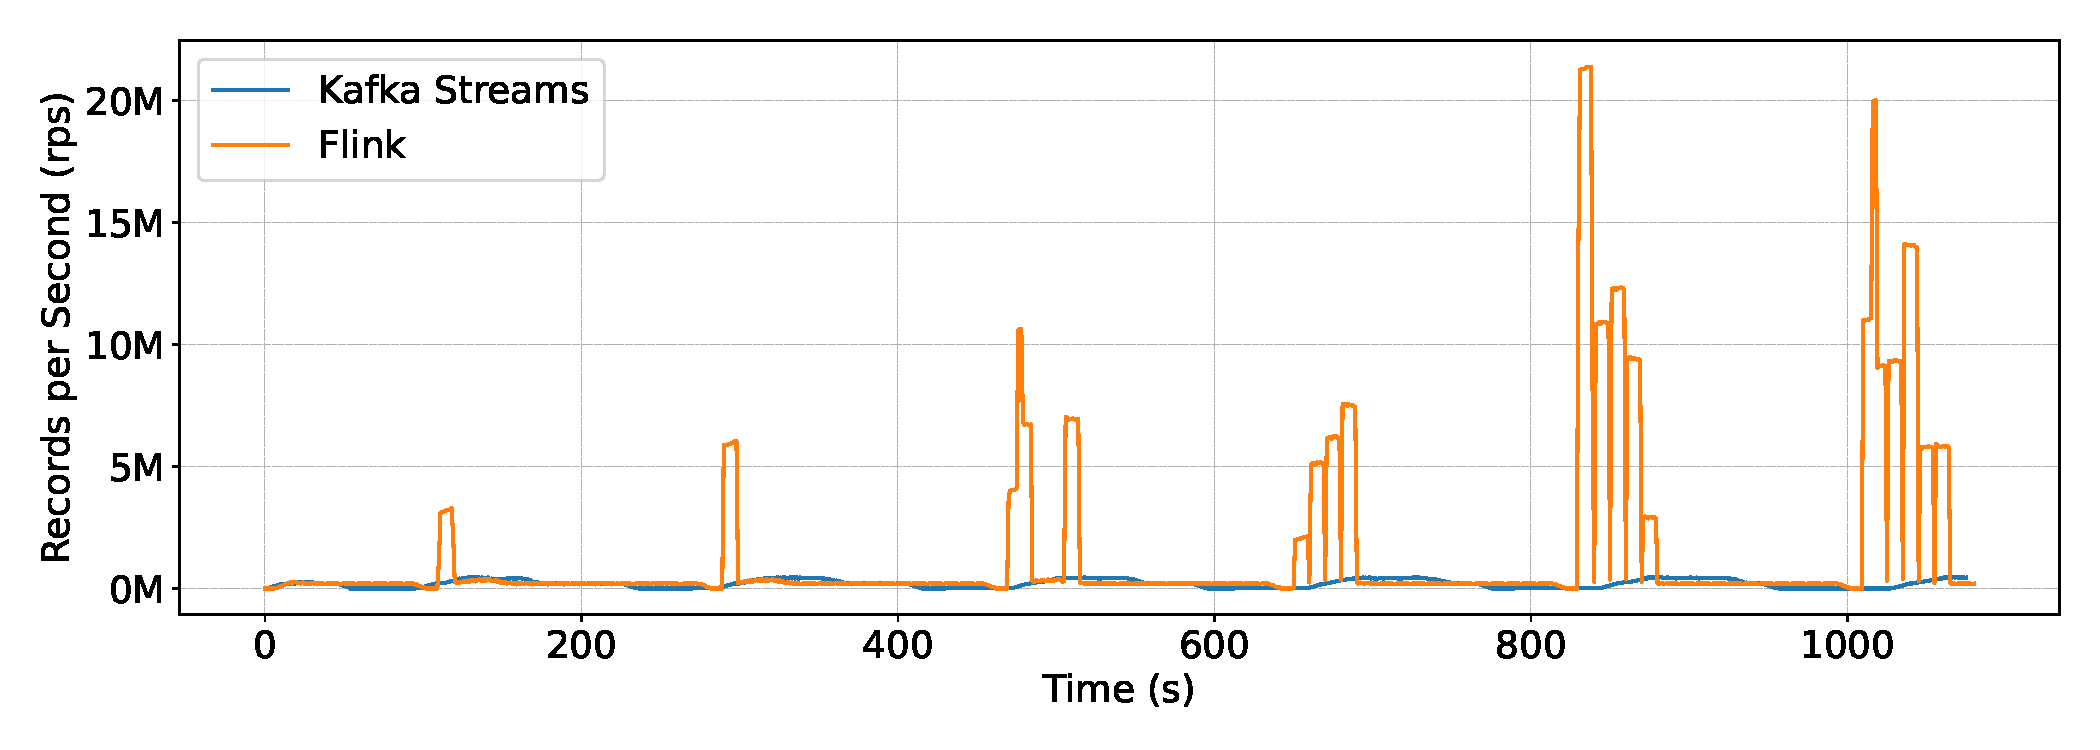
\includegraphics[width=1\textwidth]{figures/kafka-flink/input-throughput-8pod-kafka-flink}
    \caption{\textit{Input throughput for Kafka records in case of 8 workers.
    Failure period for kafka Stream and Apache Flink is not synced but happens within the same period.}}
    \label{fig:kafka-flink-input-8}
\end{figure}


In both cases on Figure \ref{fig:kafka-flink-input-2} and Figure \ref{fig:kafka-flink-input-8}
Flink is showing extreme high input rate comparing to Kafka Streams.
Flink uses its own offset commit mechanism in case of fault tolerance \cite{flink_kafka_offset}.
Also, such behavior is due to faster startup time for Flink workers, CPU metrics
on Figures \ref{fig:flink-8pods-resource} \ref{fig:flink-2pods-resource} for Flink
and on Figures \ref{fig:kafka-2pods-resource} \ref{fig:kafka-8pods-resource} for Kafka Streams
show that Flink workers get started faster.


\subsection{Output throughput}\label{subsec:output-throughtput}

\begin{figure}[H]
    \centering
    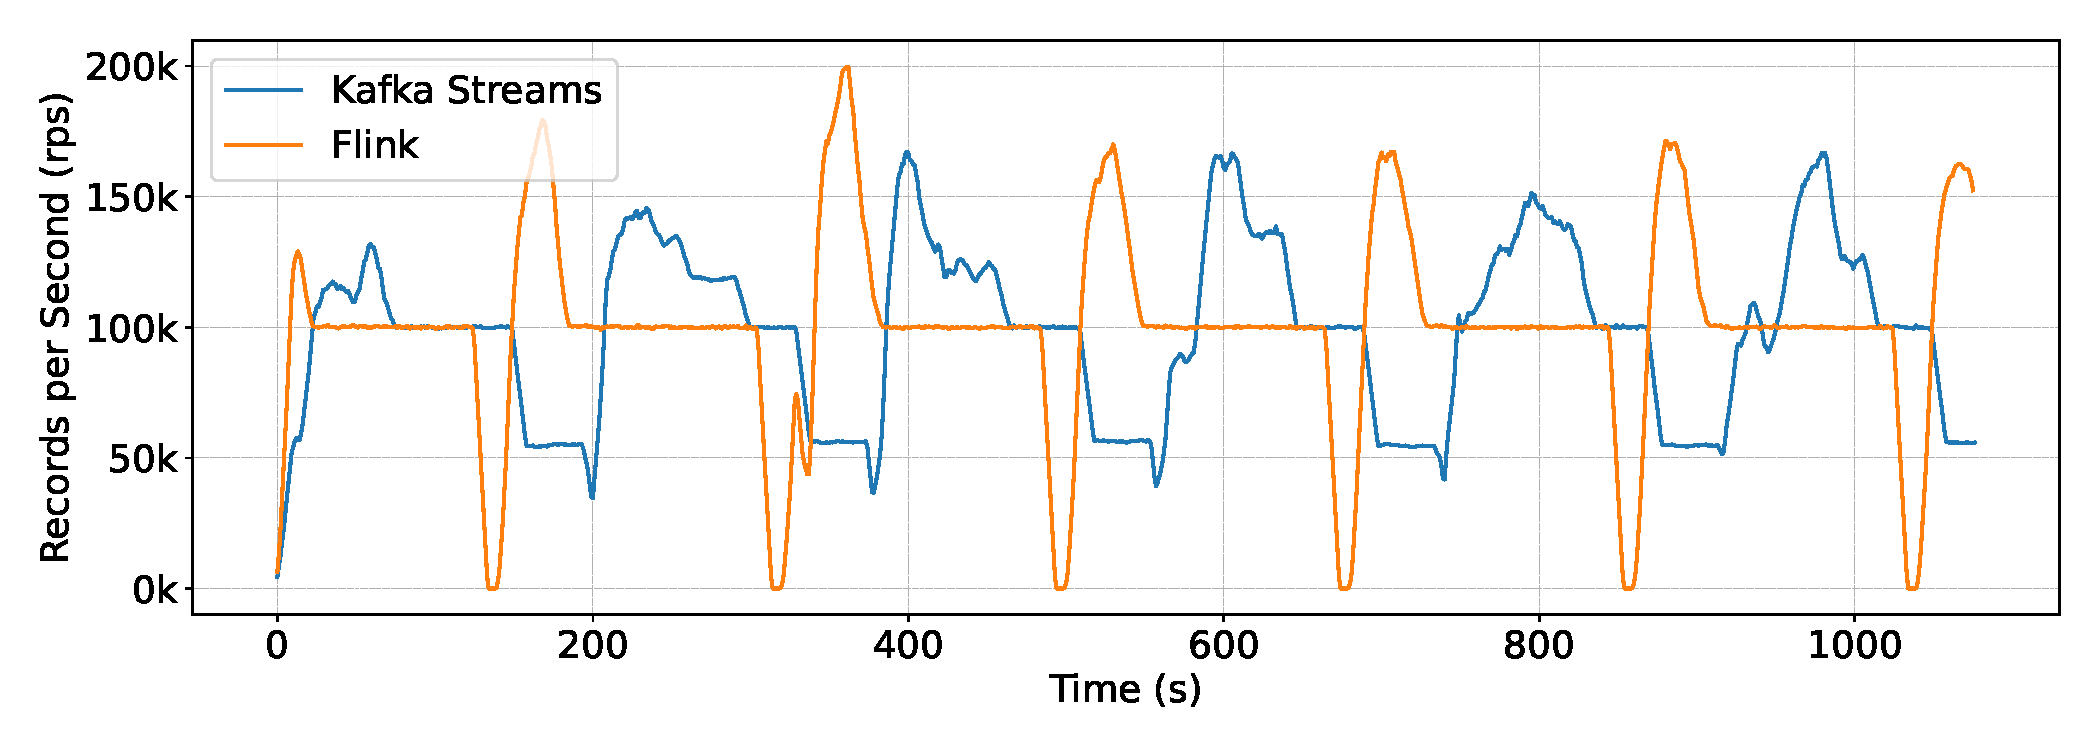
\includegraphics[width=1\textwidth]{figures/kafka-flink/output-throught-2pods-kafka-flink}
    \caption{\textit{Output throughput for Kafka records in case of 2 workers failures.
    Failure period for kafka Stream and Apache Flink is not synced but happens within the same period.}}
    \label{fig:kafka-flink-out-2}
\end{figure}


\begin{figure}[H]
    \centering
    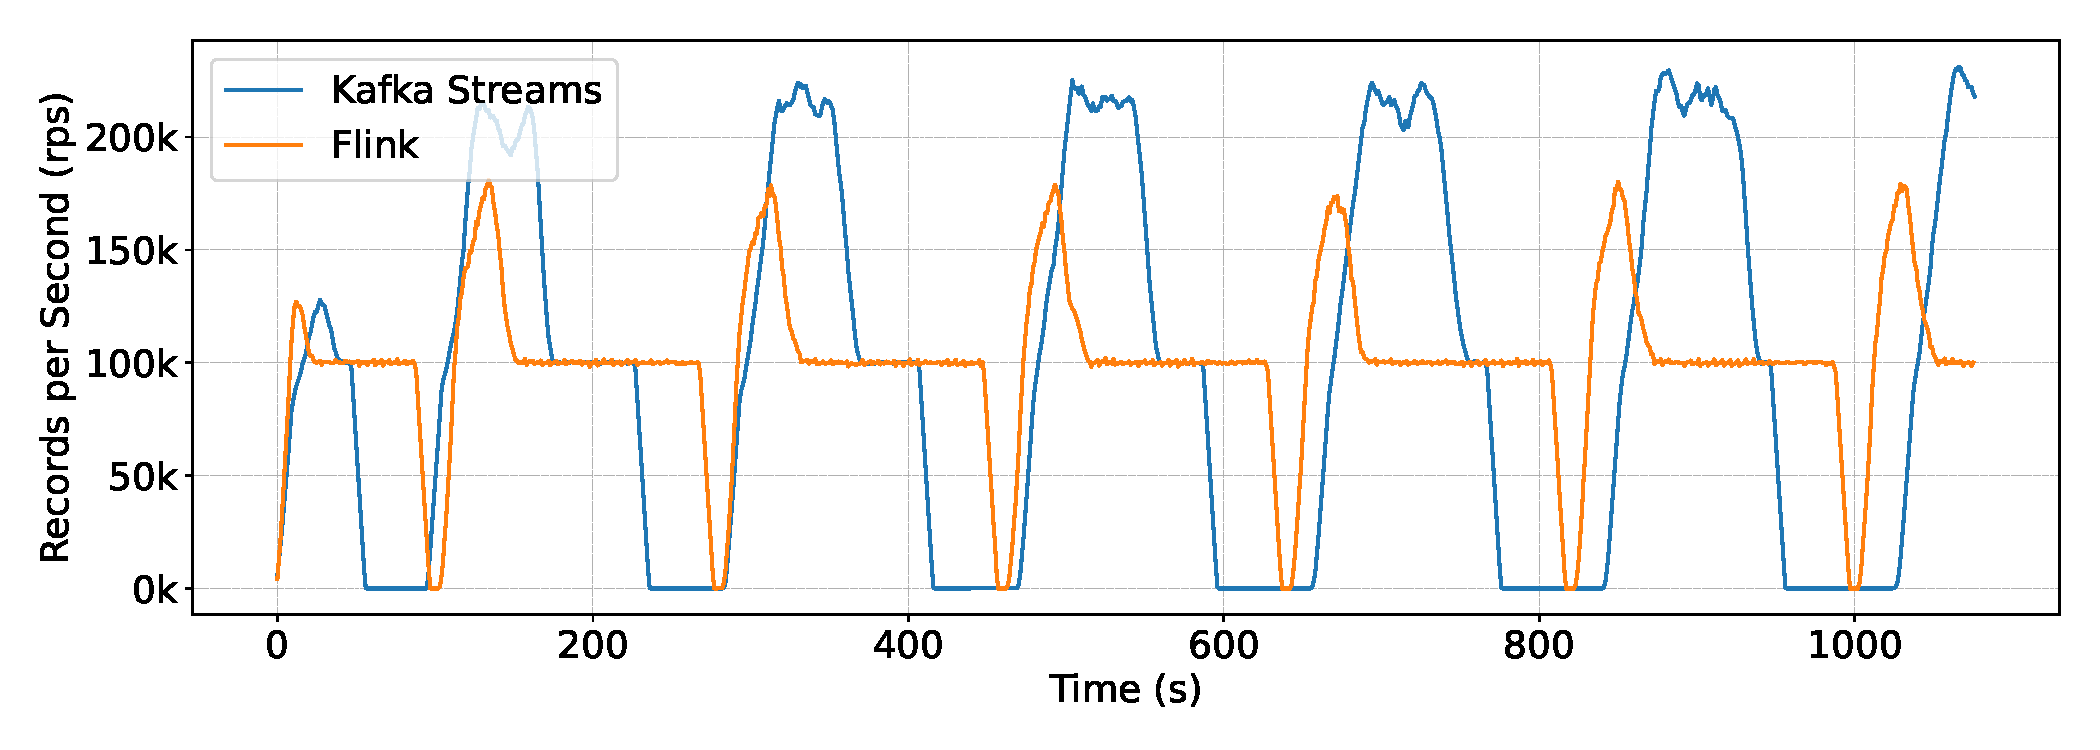
\includegraphics[width=1\textwidth]{figures/kafka-flink/output-throught-8pods-kafka-flink}
    \caption{\textit{Output throughput for Kafka records in case of 8 worker failures.
    Failure period for kafka Stream and Apache Flink is not synced but happens within the same period.}}
    \label{fig:kafka-flink-out-8}
\end{figure}

Interesting behavior can be seen on Figure \ref{fig:kafka-flink-out-2} and \ref{fig:kafka-flink-out-8}.
On the Figure \ref{fig:kafka-flink-out-2} Flink workers produce higher output rate
rather than Apache Flink while on Figure \ref{fig:kafka-flink-out-8} Kafka Streams produce
higher rate.
This behavioral could be described in the following way.
Since CPU metrics show that Kafka Streams workers need more startup time, especially
if a whole worker cluster was down for a short period.
During a downtime time, the load generator has produced a lot of uncommited records,
that Kafka Streams workers start processing later comparing to Flink.
To catch up with real time and process delayed records, Kafka Streams has to process
more records that lead to a higher output.
In the case of 2 workers downtime, Kafka Streams need to wait only for 2 worker.
Flink is able to start processing records sooner, for this reason, Flink needs to
process less uncommited records.

\newpage
\subsection{Lag trend}\label{subsec:lag-trend}
Lag trend metric is described in the benchmarks section \ref{subsec:definition-of-benchmarks}.

\begin{figure}[H]
    \centering
    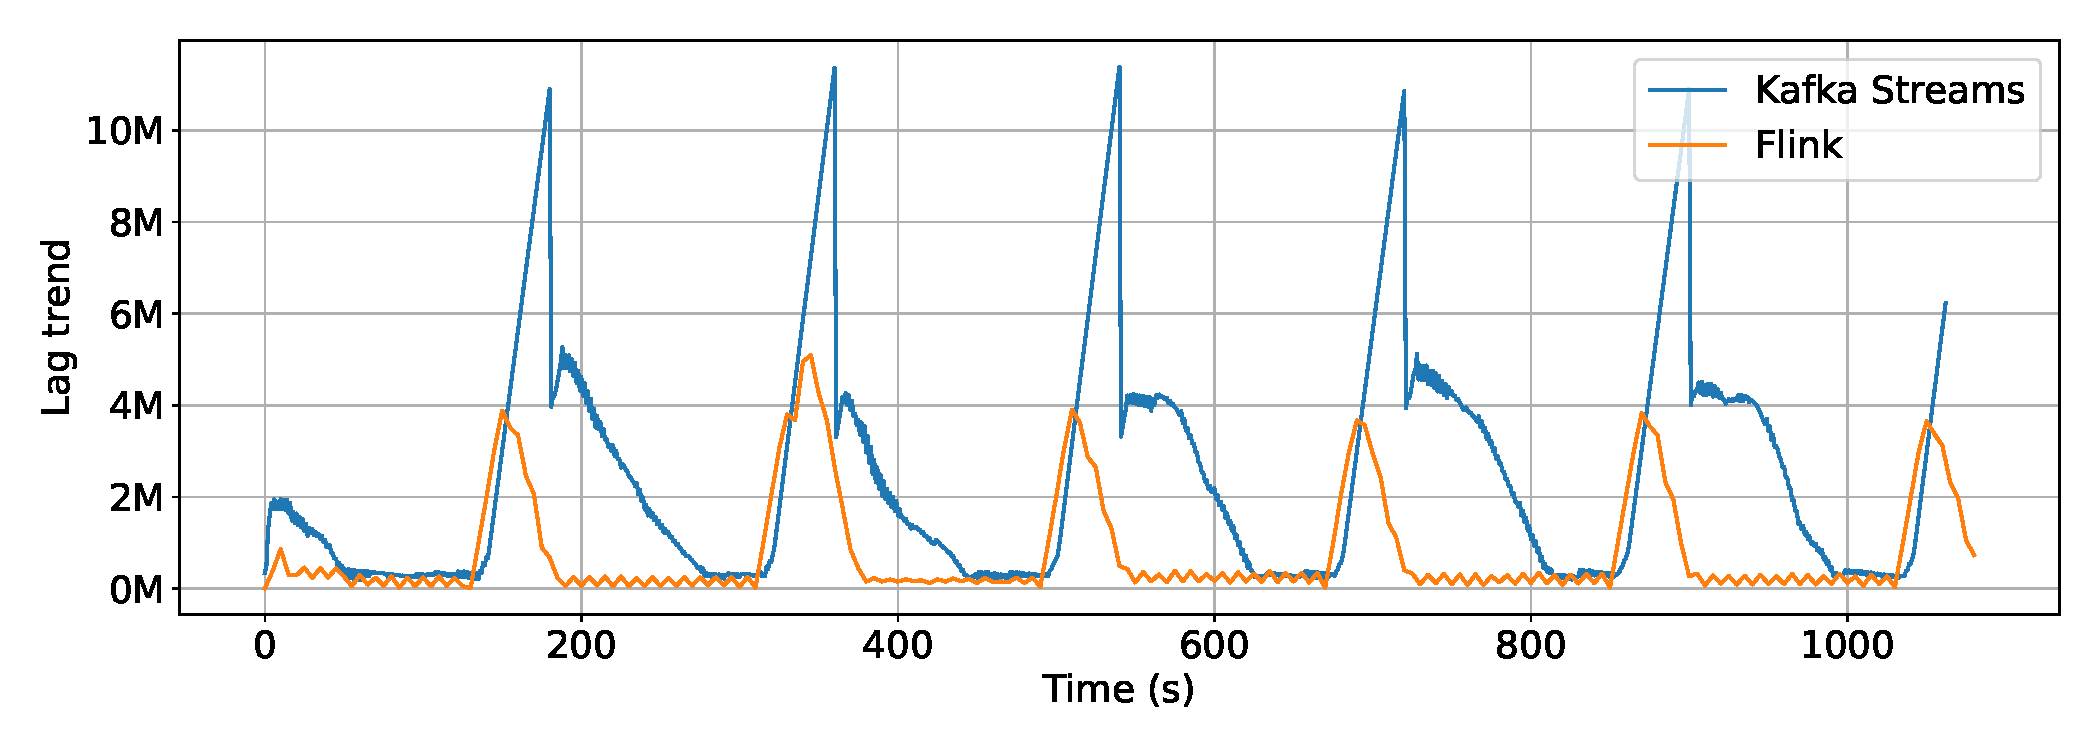
\includegraphics[width=1\textwidth]{figures/kafka-flink/lag-trend-2pod-kafka-flink}
    \caption{\textit{Lag trend for worker cluster consumer group in case of 2 worker failures.
    Failure period for kafka Stream and Apache Flink is not synced but happens within the same period.}}
    \label{fig:kafka-flink-lag-2}
\end{figure}


\begin{figure}[H]
    \centering
    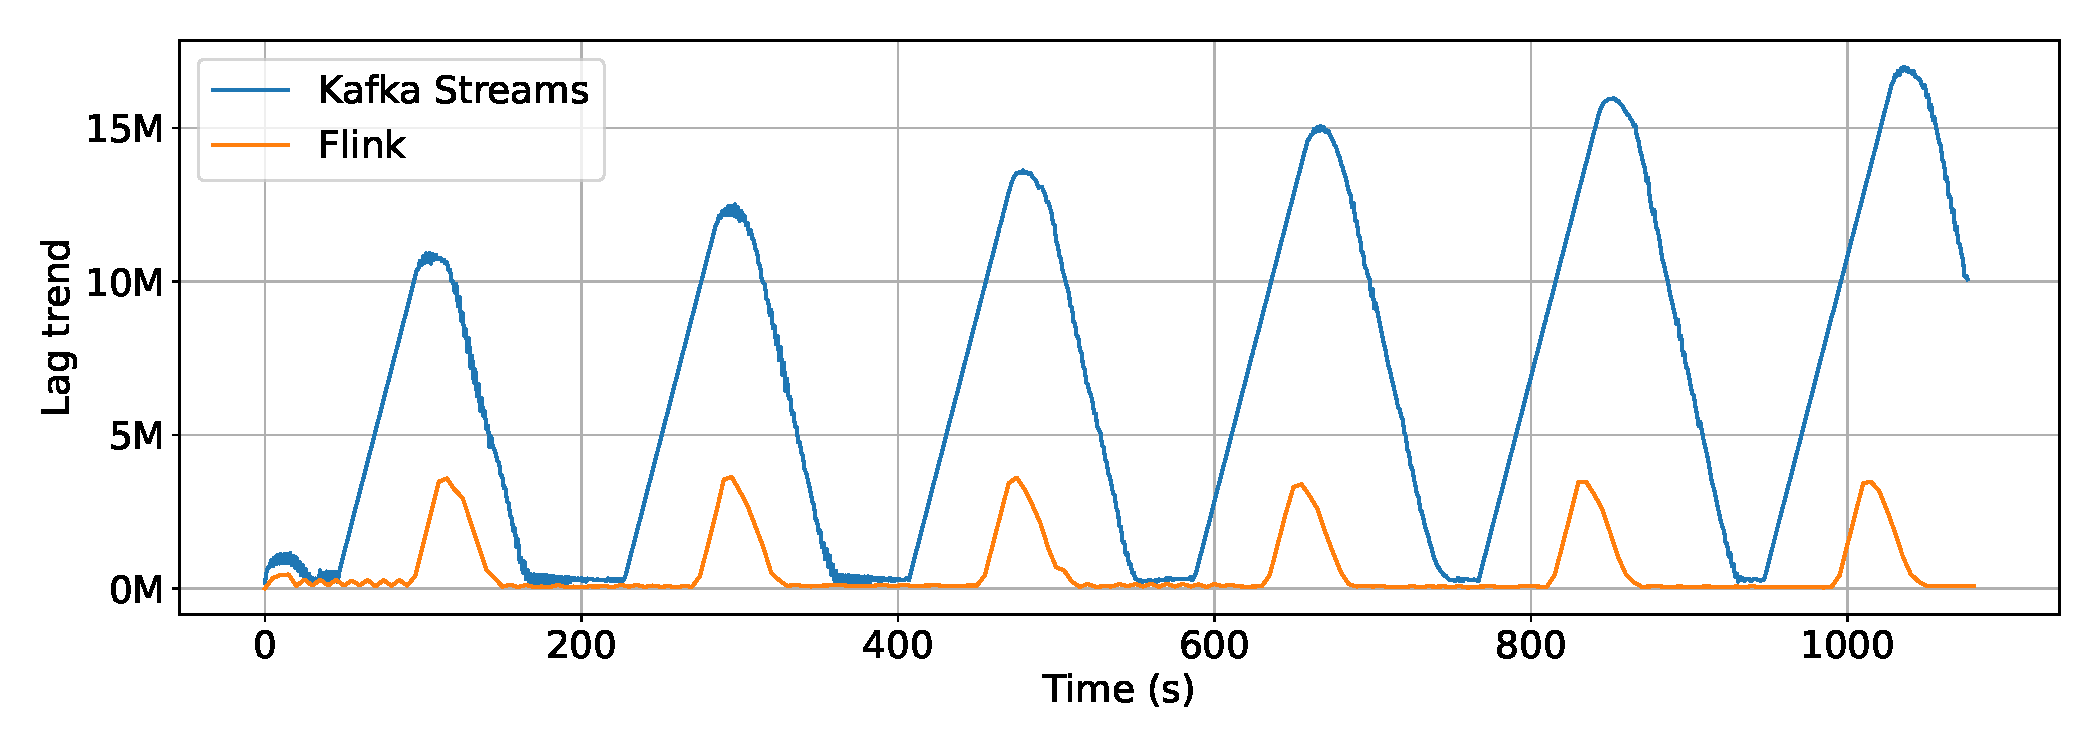
\includegraphics[width=1\textwidth]{figures/kafka-flink/lag-trend-8pod-kafka-flink}
    \caption{\textit{Lag trend for worker cluster consumer group in case of 8 worker failures.
    Failure period for kafka Stream and Apache Flink is not synced but happens within the same period.}}
    \label{fig:kafka-flink-lag-8}
\end{figure}

As described in \ref{subsec:output-throughtput}, due to faster startup time
and different records offset processing, Flink is able to process
input records with less delay.
For this reason, there is such a lag difference on Figure \ref{fig:kafka-flink-lag-2} and Figure \ref{fig:kafka-flink-lag-8}.

\newpage
\subsection{CPU utilization}\label{subsec:cpu-utilization}

\begin{figure}[H]
    \centering
    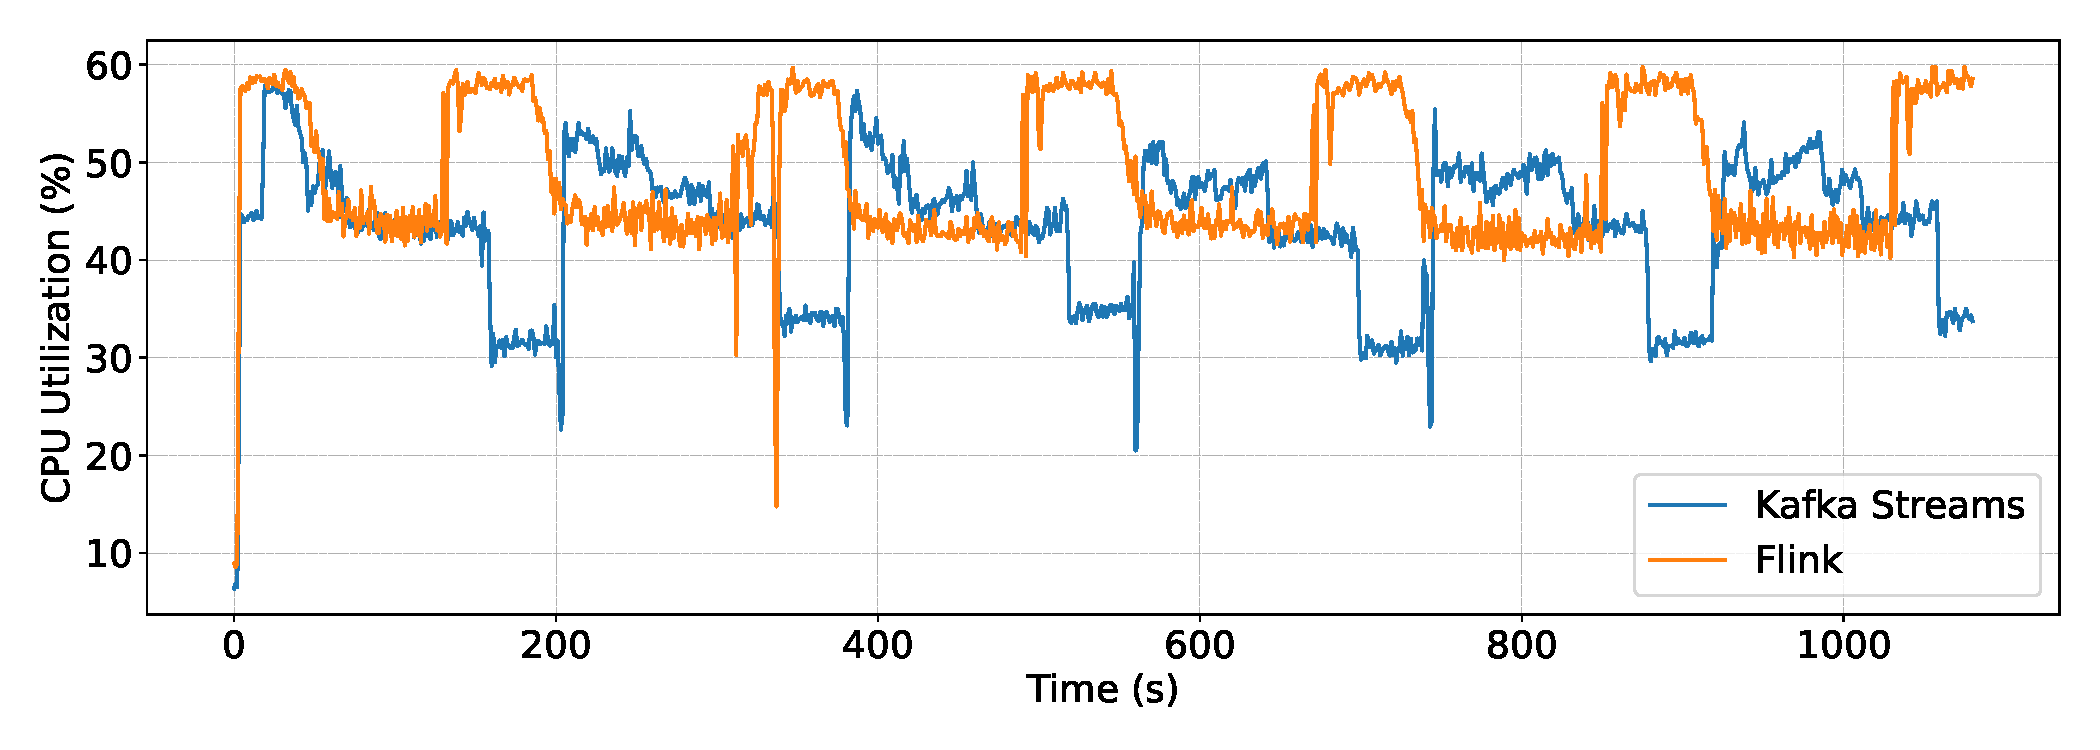
\includegraphics[width=1\textwidth]{figures/kafka-flink/cpu-utilization-2pods-kafka-flink}
    \caption{\textit{Average CPU utilization for all workers in case of 2 worker failures.
    Failure period for kafka Stream and Apache Flink is not synced but happens within the same period.}}
    \label{fig:kafka-flink-cpu-2}
\end{figure}


\begin{figure}[H]
    \centering
    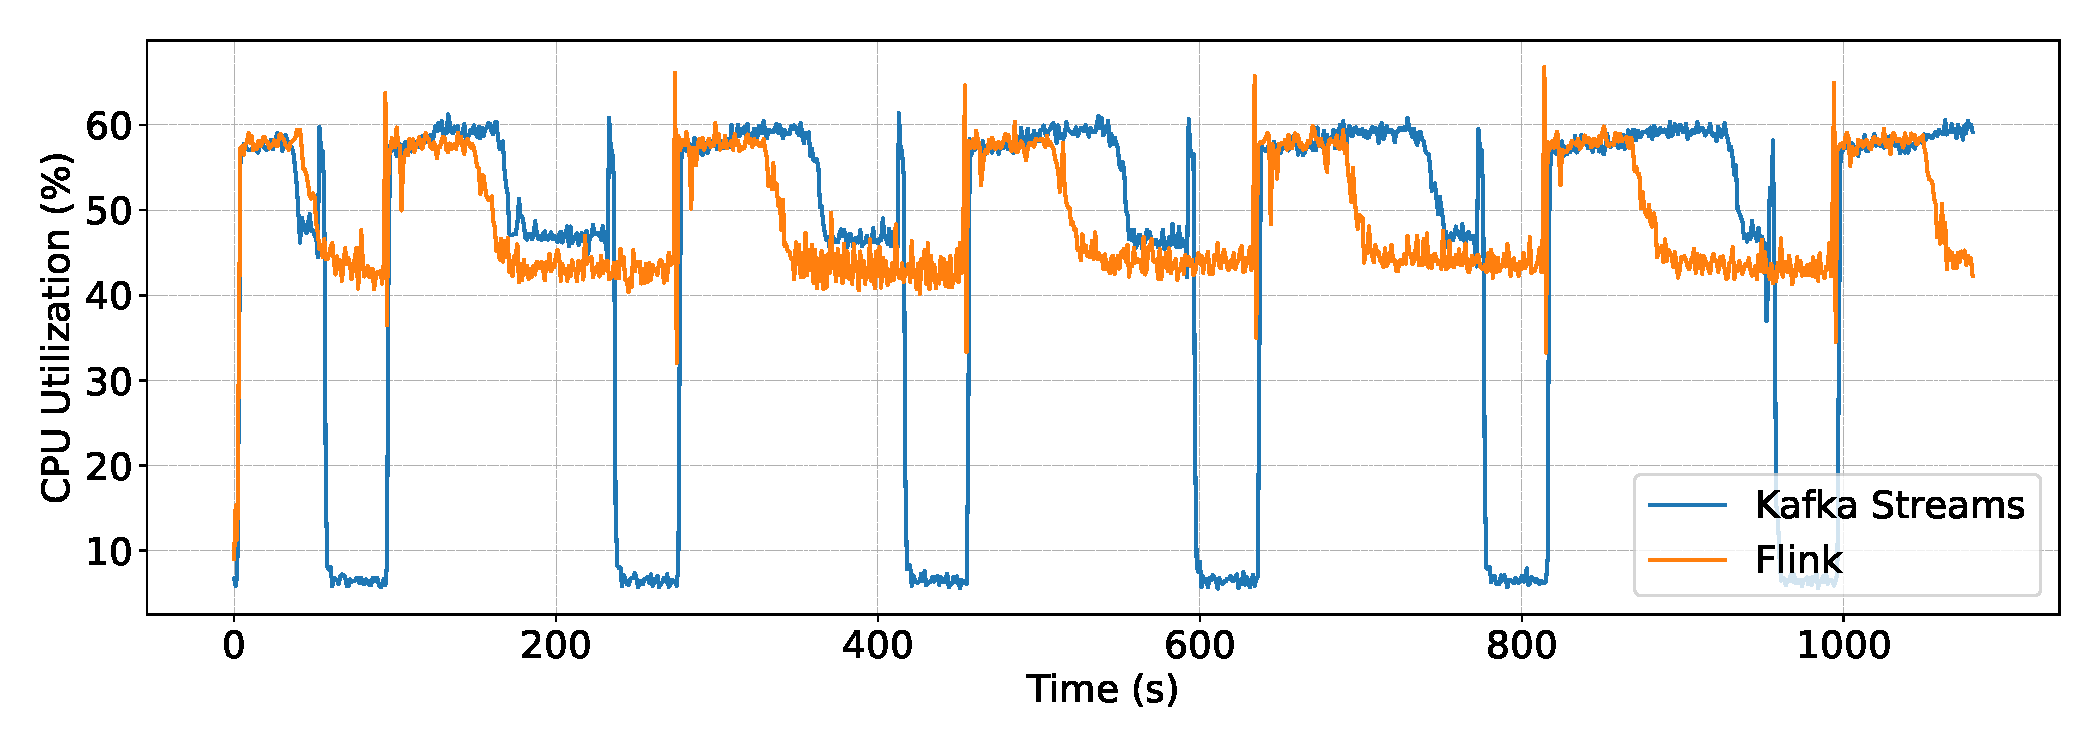
\includegraphics[width=1\textwidth]{figures/kafka-flink/cpu-utilization-8pods-kafka-flink}
    \caption{\textit{Average CPU utilization for all workers in case of 8 worker failures.
    Failure period for kafka Stream and Apache Flink is not synced but happens within the same period.}}
    \label{fig:kafka-flink-cpu-8}
\end{figure}

CPU metrics on Figure \ref{fig:kafka-flink-cpu-2} and \ref{fig:kafka-flink-cpu-8}
show faster Flink workers startup for both cases.
Kafka Streams workers show higher downtime.


\newpage
\subsection{Network traffic}\label{subsec:inbound-network}

\begin{figure}[H]
    \centering
    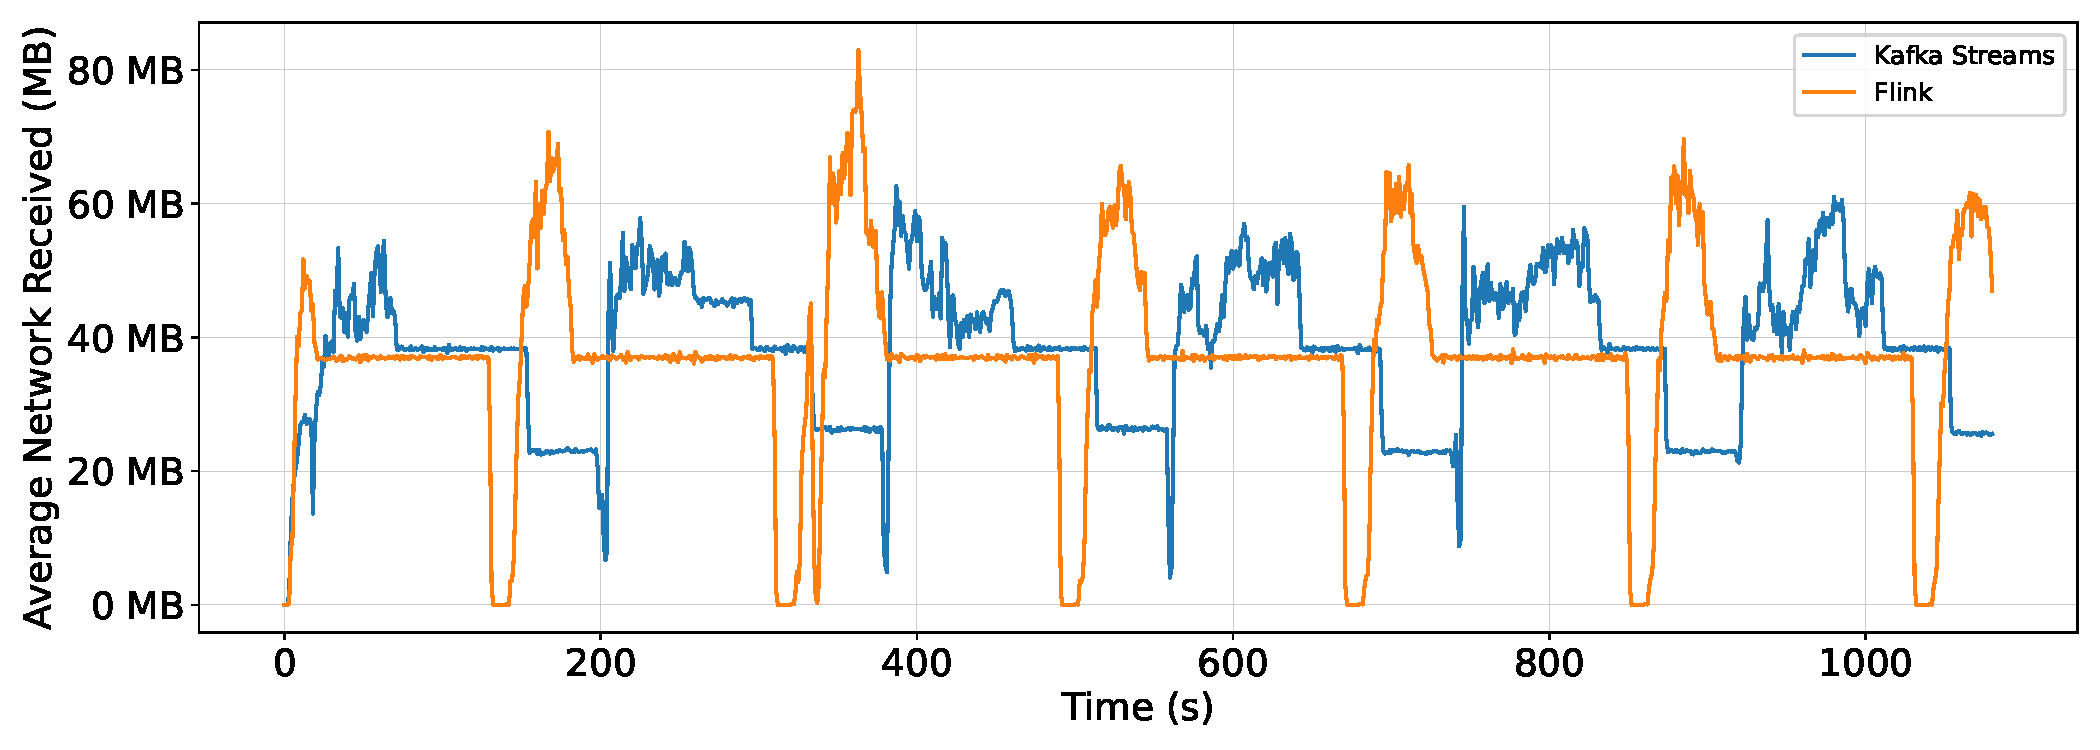
\includegraphics[width=1\textwidth]{figures/kafka-flink/network-received-2pod-kafka-flink}
    \caption{\textit{Average inbound network traffic for all workers in case of 2 worker failures.
    Failure period for kafka Stream and Apache Flink is not synced but happens within the same period.}}
    \label{fig:kafka-flink-received-2}
\end{figure}


\begin{figure}[H]
    \centering
    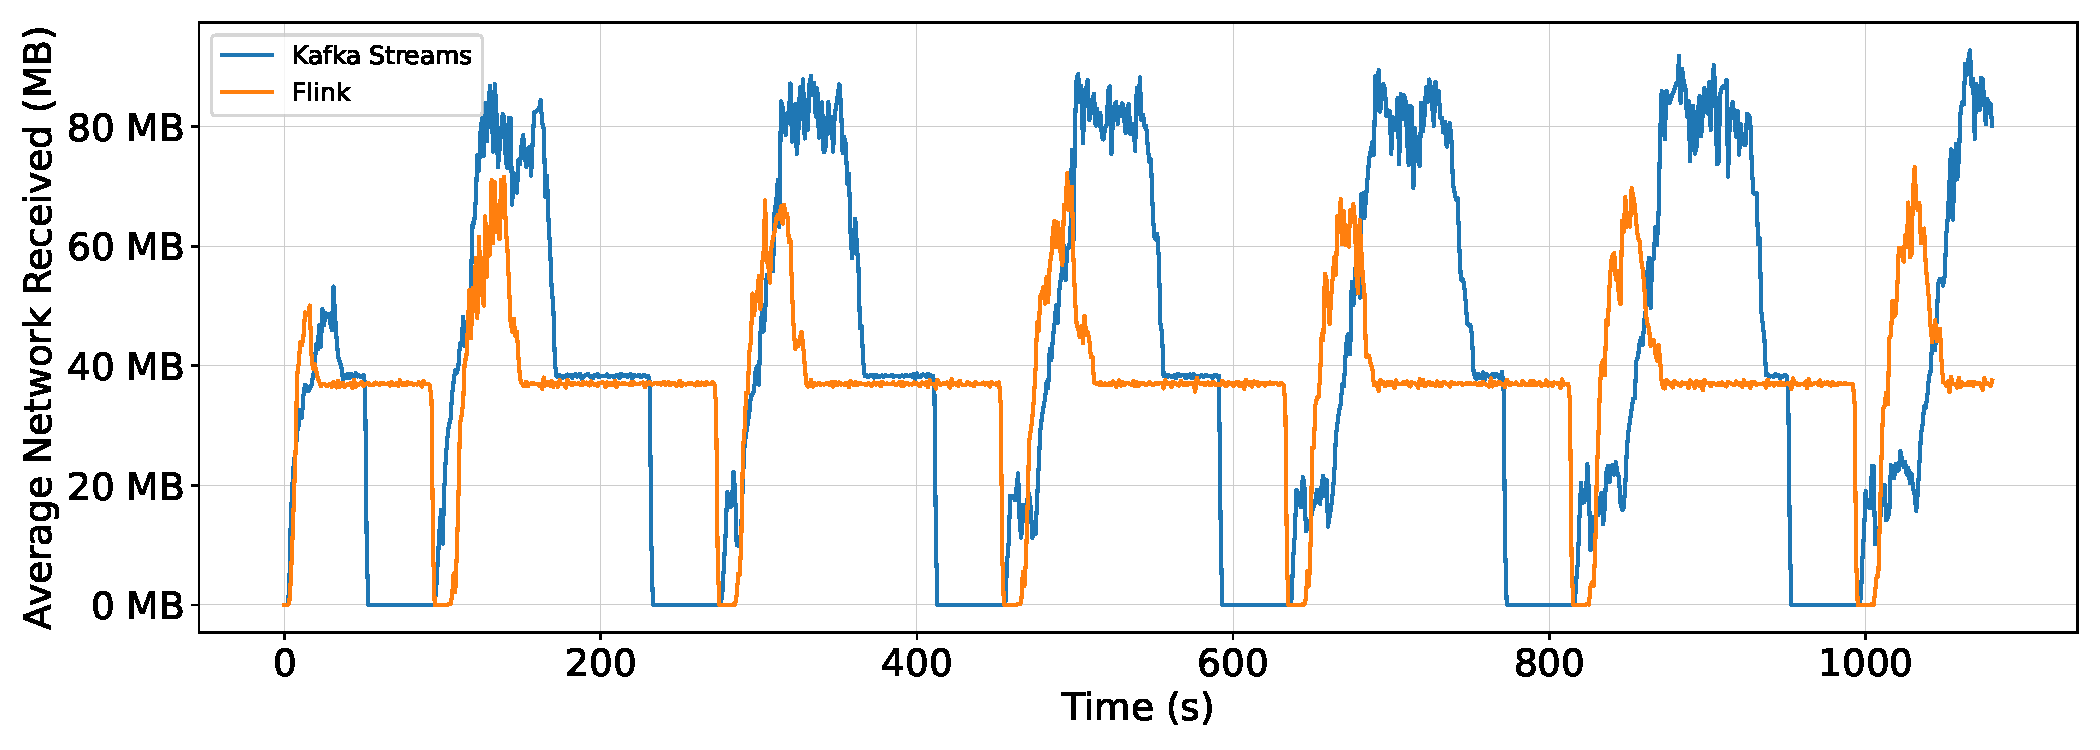
\includegraphics[width=1\textwidth]{figures/kafka-flink/network-received-8pod-kafka-flink}
    \caption{\textit{Average inbound network traffic for all workers in case of 8 worker failures.
    Failure period for kafka Stream and Apache Flink is not synced but happens within the same period.}}
    \label{fig:kafka-flink-received-8}
\end{figure}

\begin{figure}[H]
    \centering
    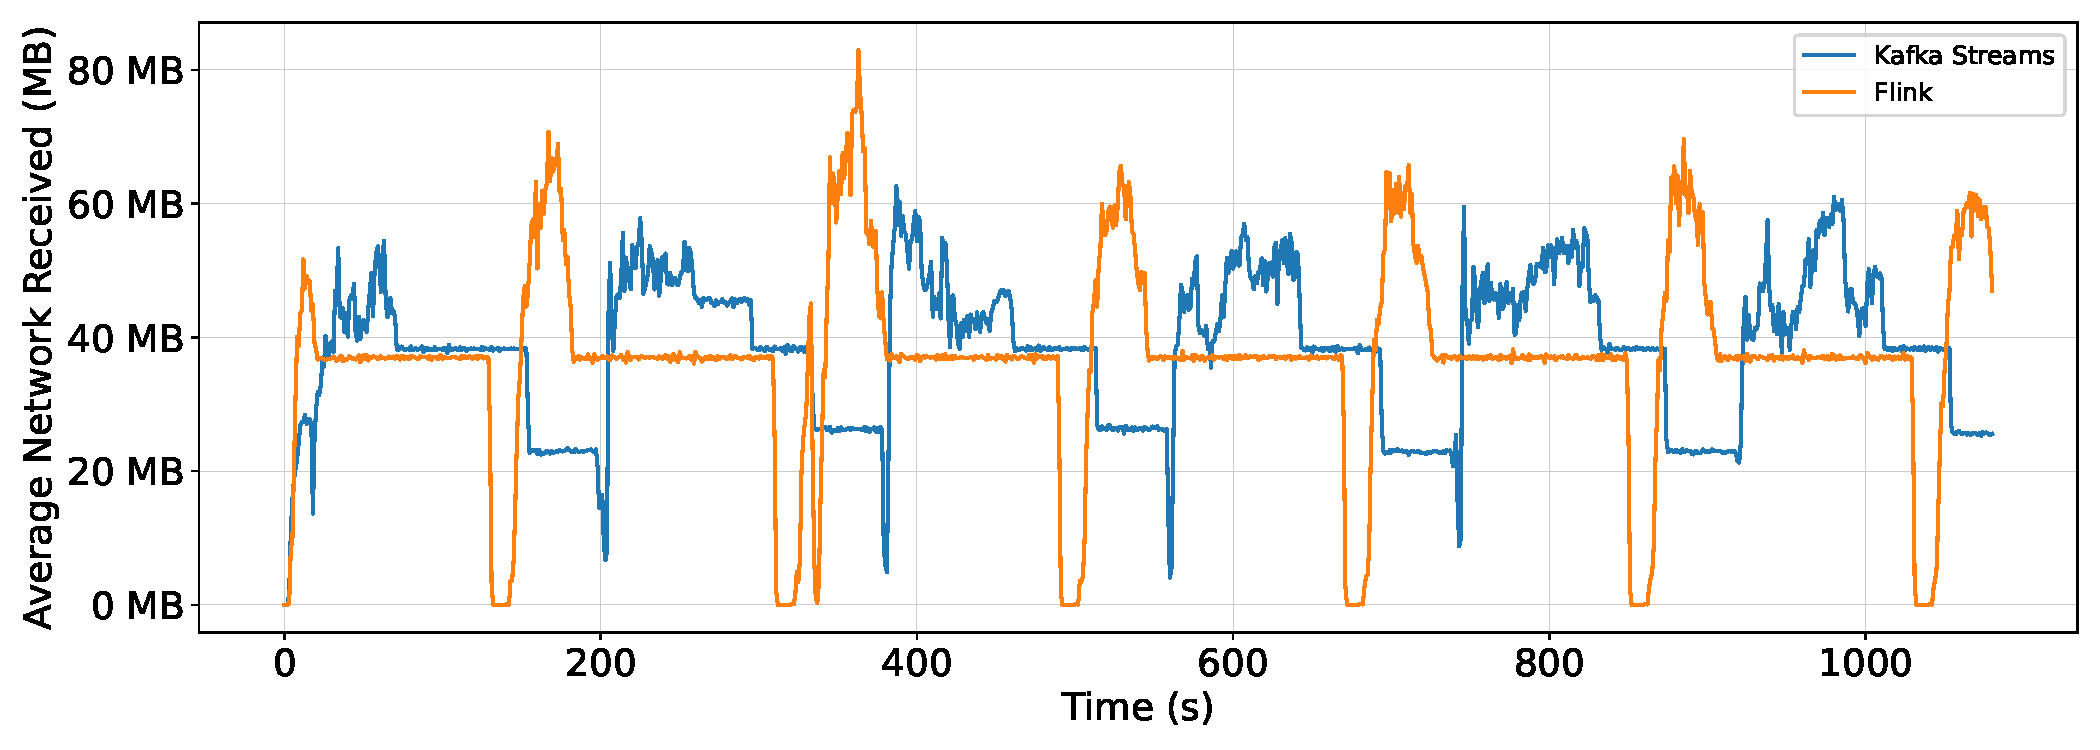
\includegraphics[width=1\textwidth]{figures/kafka-flink/network-received-2pod-kafka-flink}
    \caption{\textit{Average outbound network traffic for all workers in case of 2 worker failures.
    Failure period for kafka Stream and Apache Flink is not synced but happens within the same period.}}
    \label{fig:kafka-flink-transmitted-2}
\end{figure}


\begin{figure}[H]
    \centering
    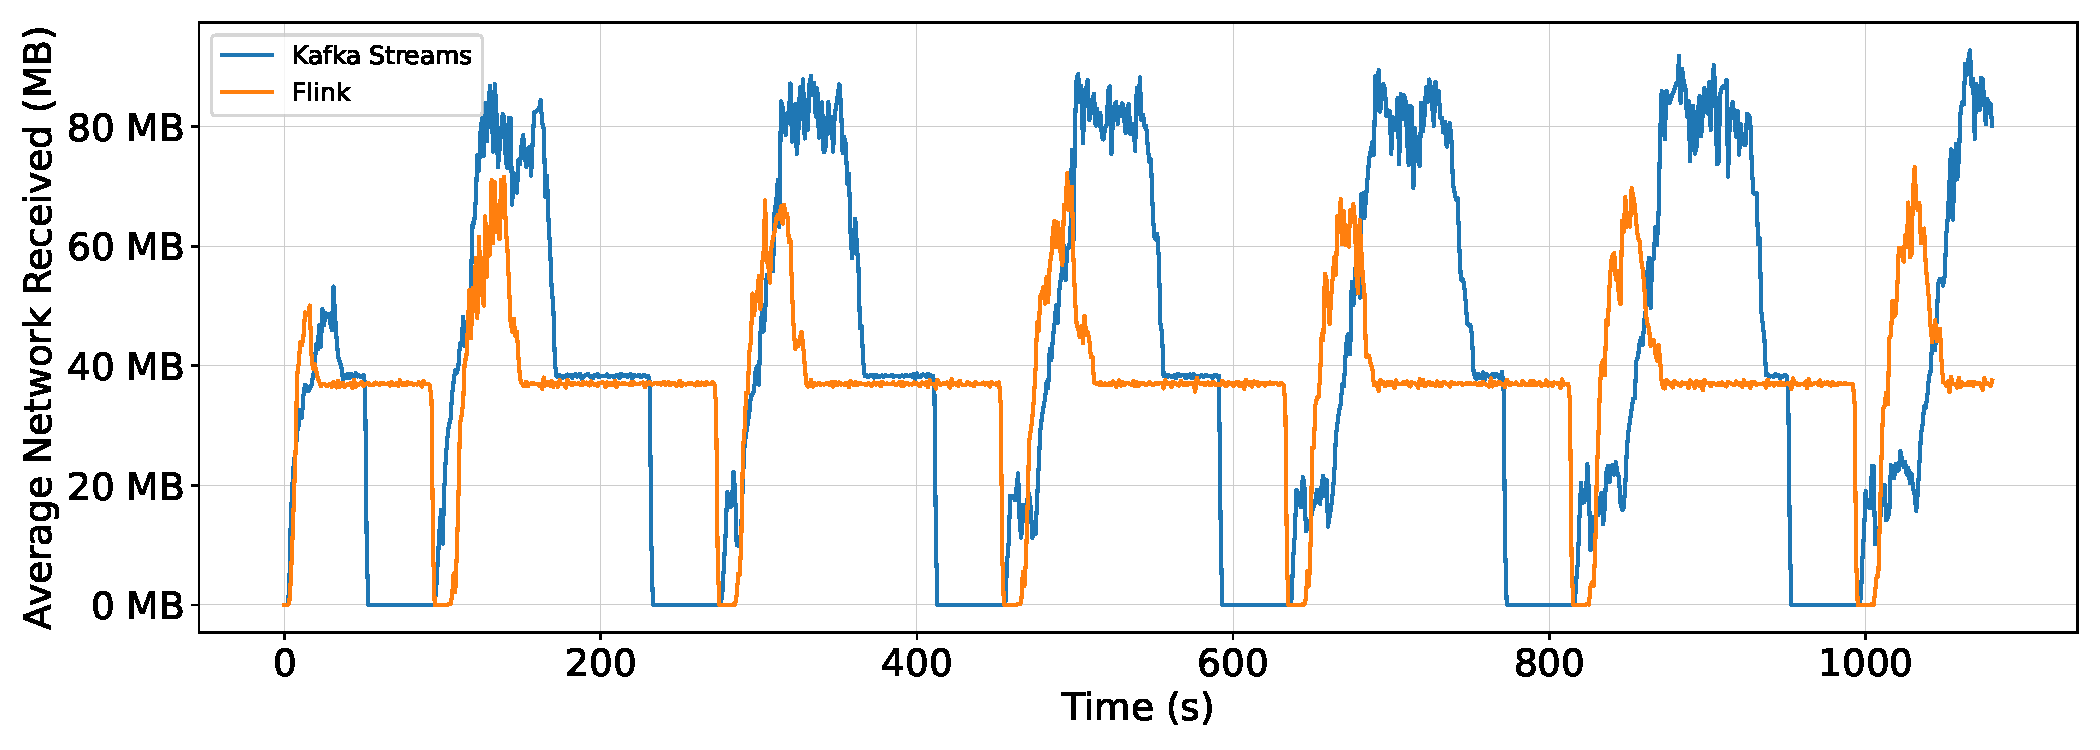
\includegraphics[width=1\textwidth]{figures/kafka-flink/network-received-8pod-kafka-flink}
    \caption{\textit{Average outbound network traffic for all workers in case of 8 worker failures.
    Failure period for kafka Stream and Apache Flink is not synced but happens within the same period.}}
    \label{fig:kafka-flink-transmitted-8}
\end{figure}

Inbound and outbound network traffic is used for a state recovery and
incoming load processing.
In case of 8 worker failures Figure \ref{fig:kafka-flink-received-8} and Figure \ref{fig:kafka-flink-transmitted-8}
Kafka Streams uses higher network to process faster uncommited records during the downtime.
Output record rate on Figure  \ref{fig:kafka-8pods-impact} is higher to due to longer downtime for
Kafka Streams workers.
However, Flink workers show high spikes in case of 2 worker failures, but for a shorter period.